% OBJETIVO DEL CAPÍTULO: Reflejar una progresión impecable desde 
% la matemática pura (Variedades) -> Topología aplicada (Obstáculos/Recubrimientos) 
% -> Computación (Algoritmos en Python) -> Validación física (Análisis Diferencial).

\section{Fundamentos de la robótica topológica}
% NOTA DE ESTRATEGIA: Introducimos a Farber y Munkres, y construimos el "tablero de juego" (el Toro) 
% antes de poner al robot a moverse.
La robótica topológica proporciona el marco matemático necesario para comprender 
el movimiento de los manipuladores más allá de la simple cinemática local. 
Antes de implementar algoritmos de búsqueda, es imperativo formalizar el \enquote{tablero de juego} 
donde opera el robot. En esta sección, se establecen los conceptos fundamentales que 
permiten abstraer la estructura física del manipulador hacia una variedad matemática, 
definiendo las reglas de continuidad y conectividad que gobernarán la planificación de 
trayectorias.



\subsection{Espacios topológicos y variedades diferenciables}
% - Definición formal de espacio topológico y espacio métrico.

Para formalizar el espacio en el que opera el manipulador, es necesario establecer 
las bases matemáticas de su geometría y continuidad, partiendo desde los conceptos más 
estrictos de medición hasta la generalización topológica.

\begin{definition}[Espacio Métrico]
Un espacio métrico se define como un par ordenado $(X, d)$, donde $X$ es un 
conjunto no vacío y $d: X \times X \to \mathbb{R}$ es una función denominada 
métrica o distancia. Para que $d$ sea considerada una métrica, debe satisfacer 
los siguientes tres axiomas para cualesquiera elementos $x, y, z \in X$ \parencite{antonyan2016topologia}:

\begin{enumerate}
    \item \textbf{Positividad:} $d(x, y) \ge 0$, cumpliéndose que $d(x, y) = 0$ si y solo si $x = y$.
    \item \textbf{Simetría:} $d(x, y) = d(y, x)$.
    \item \textbf{Desigualdad del triángulo:} $d(x, z) \le d(x, y) + d(y, z)$.
\end{enumerate}

En este contexto, al valor real arrojado por $d(x, y)$ se le conoce formalmente 
como la distancia métrica entre los puntos $x$ e $y$.
\end{definition}

\begin{definition}[Espacio Topológico]

Un espacio topológico se formaliza como un par $(X, \tau)$, donde $X$ es un 
conjunto no vacío y $\tau$ representa una familia de subconjuntos de $X$. Los elementos 
que conforman $\tau$ reciben el nombre de \textit{conjuntos abiertos}, y para que esta 
estructura sea matemáticamente válida, debe cumplir de forma estricta con tres axiomas 
fundamentales \parencite{antonyan2016topologia}:

\begin{enumerate}
    \item \textbf{Contención elemental:} Tanto el conjunto vacío ($\emptyset$) como el espacio 
    total ($X$) pertenecen a la colección $\tau$.
    \item \textbf{Uniones arbitrarias:} Si $\{U_\alpha\}_{\alpha \in A}$ es una familia 
    cualquiera (ya sea finita o infinita) de conjuntos en $\tau$, su 
    unión $\bigcup_{\alpha \in A} U_\alpha$ también pertenece a $\tau$.
    \item \textbf{Intersecciones finitas:} Si $\{U_1, \dots, U_n\}$ es una familia 
    finita de elementos en $\tau$, su intersección $\bigcap_{i=1}^n U_i$ necesariamente 
    pertenece a $\tau$.
\end{enumerate}
\end{definition}

La relación intrínseca entre ambas estructuras radica en que todo espacio métrico $(X, d)$ 
induce de manera natural un espacio topológico $(X, \tau_d)$. En este caso, la 
topología $\tau_d$ es generada por las bolas abiertas que se derivan directamente de su 
función de distancia \parencite{antonyan2016topologia}. 

La principal ventaja analítica de abstraer el problema hacia la teoría de espacios 
topológicos es que permite generalizar conceptos cruciales, como la proximidad 
y la continuidad de trayectorias, en entornos complejos donde no existe una 
función de distancia euclidiana evidente \parencite{waldmann2014topology}. Sin embargo, 
esta abstracción presenta la desventaja de perder las propiedades geométricas explícitas; 
al omitir una métrica estricta, no es posible calcular de manera directa la longitud de 
una ruta, lo cual exigirá posteriormente la reintroducción de funciones de 
distancia específicas (como las métricas $L_1$ y $L_2$) para evaluar y optimizar 
el costo del movimiento del robot.


% - Introducción a las variedades (manifolds): el concepto de ser "localmente euclidiano" (cartas y atlas).
% - Propósito: Preparar el terreno para justificar el uso de herramientas de \mathbb{R}^n en espacios curvos.
Para resolver esta disyuntiva, preservar la flexibilidad analítica global mientras se recupera la capacidad de medición 
y cálculo, es necesario estructurar el problema bajo un marco matemático intermedio. Es aquí donde surge la idea 
fundamental detrás de una variedad topológica (o \textit{manifold}): describir un espacio que, aunque globalmente 
pueda poseer una topología compleja o curva, a nivel local se ve y se comporta de manera idéntica a un subconjunto 
abierto del espacio euclidiano $\mathbb{R}^n$. Para formalizar matemáticamente esta noción de ser localmente euclidiano, 
es indispensable introducir los siguientes constructos geométricos \parencite{waldmann2014topology}:

\begin{itemize}
    \item \textbf{Cartas locales:} Sea $(M, \tau)$ un espacio topológico 
    y $U \subseteq M$ un subconjunto abierto. Un homeomorfismo $\varphi: U \to \varphi(U) \subseteq \mathbb{R}^n$ 
    sobre un subconjunto abierto $\varphi(U)$ de $\mathbb{R}^n$ se 
    denomina una carta local de dimensión $n$ para el espacio $(M, \tau)$. 
    Esta noción es análoga a utilizar un mapa plano de una ciudad para navegar 
    sobre la superficie curva de la Tierra (véase la Figura \ref{fig:carta_local_variedad}); 
    localmente, la curvatura es despreciable 
    y la geometría euclidiana funciona perfectamente.
    
    \item \textbf{Atlas topológico:} Para describir la totalidad del espacio $M$, se 
    requiere una cubierta abierta formada por una familia de cartas locales $\{(U_i, \varphi_i)\}_{i \in I}$ 
    de tal forma que $M = \bigcup_{i \in I} U_i$.
    Siguiendo la analogía, un solo mapa no basta para representar toda la esfera 
    terrestre sin distorsión; se requiere una colección de mapas (un atlas) que 
    cubra toda la superficie solapándose entre sí.
    
    \item \textbf{Cambio de coordenadas:} Cuando dos cartas locales $(U_i, \varphi_i)$ y $(U_j, \varphi_j)$ 
    se intersectan, es decir, $U_i \cap U_j \neq \emptyset$, es analíticamente posible transitar 
    de un sistema de coordenadas a otro. La función $\phi_{ij} = \varphi_i \circ (\varphi_j|_{U_i \cap U_j})^{-1}$ 
    actúa como un homeomorfismo entre dos subconjuntos abiertos de $\mathbb{R}^n$ y se denomina mapa 
    de transición o cambio de coordenadas de la carta $j$ a la carta $i$.
\end{itemize}

Con estas herramientas establecidas, es posible asentar la definición rigurosa que constituye el 
núcleo analítico de la geometría diferencial y, por extensión, de la robótica topológica \parencite{waldmann2014topology}:

\begin{definition}[Variedad Topológica]
Un espacio topológico $(M, \tau)$ se denomina una variedad topológica de dimensión $n$ 
si satisface estrictamente las siguientes tres propiedades:
\begin{enumerate}
    \item \textbf{Localmente Euclidiano:} Para cada punto $p \in M$ existe una carta local de 
    dimensión $n$, $(U, \varphi)$, tal que $p \in U$.
    \item \textbf{Segundo numerable:} La topología $\tau$ cumple con el segundo 
    axioma de numerabilidad.
    \item \textbf{Espacio de Hausdorff:} La topología $\tau$ es de Hausdorff.
\end{enumerate}
\end{definition}

\begin{figure}[htbp]
    \centering
    % !TeX root = ../main.tex
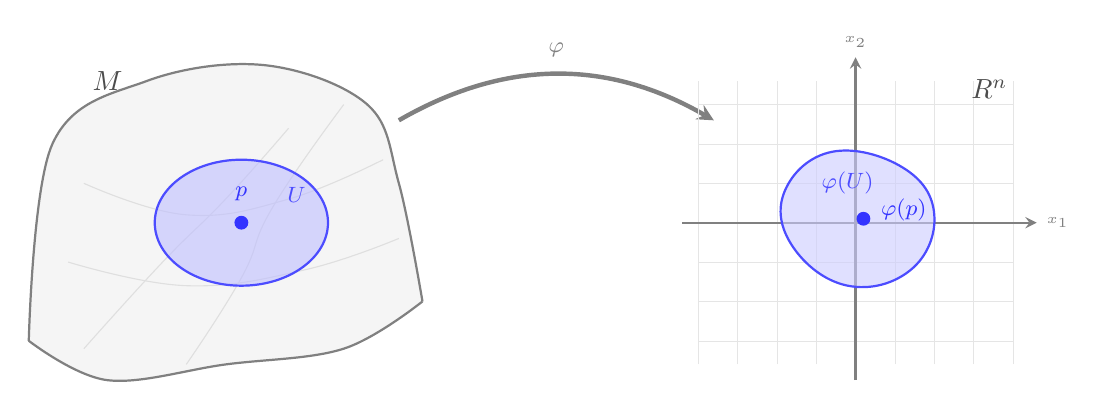
\begin{tikzpicture}[>=stealth, scale=1.0, every node/.style={font=\small}]

% =============================================
% IZQUIERDA: Variedad Topológica M
% =============================================
\begin{scope}[shift={(-4,0)}]
    % Superficie curva (simulada con un path suave)
    \fill[gray!8] 
        plot[smooth, tension=0.6] coordinates {(-2.5,-1.5) (-1.5,-2) (0,-1.8) (1.5,-1.6) (2.5,-1)}
        -- plot[smooth, tension=0.6] coordinates {(2.5,-1) (2.2,0.5) (1.8,1.5) (0.5,2) (-1,1.8) (-2.2,1) (-2.5,-1.5)};
    \draw[black!50, thick] 
        plot[smooth, tension=0.6] coordinates {(-2.5,-1.5) (-1.5,-2) (0,-1.8) (1.5,-1.6) (2.5,-1)};
    \draw[black!50, thick] 
        plot[smooth, tension=0.6] coordinates {(2.5,-1) (2.2,0.5) (1.8,1.5) (0.5,2) (-1,1.8) (-2.2,1) (-2.5,-1.5)};
    
    % Líneas de curvatura (dan profundidad)
    \draw[gray!25, thin] 
        plot[smooth, tension=0.8] coordinates {(-1.8,-1.6) (-0.8,-0.5) (0,0.3) (0.8,1.2)};
    \draw[gray!25, thin] 
        plot[smooth, tension=0.8] coordinates {(-0.5,-1.8) (0.2,-0.7) (0.6,0.2) (1.5,1.5)};
    \draw[gray!25, thin] 
        plot[smooth, tension=0.7] coordinates {(-2.0,-0.5) (-0.5,-0.8) (1.0,-0.6) (2.2,-0.2)};
    \draw[gray!25, thin] 
        plot[smooth, tension=0.7] coordinates {(-1.8,0.5) (-0.5,0.1) (0.8,0.3) (2.0,0.8)};
    
    % Vecindad U (elipse resaltada sobre la superficie)
    \fill[blue!25, opacity=0.6] (0.2,0) ellipse (1.1 and 0.8);
    \draw[blue!70, thick] (0.2,0) ellipse (1.1 and 0.8);
    
    % Punto p
    \fill[blue!80] (0.2,0) circle (2.5pt);
    \node[font=\footnotesize, blue!80, anchor=south] at (0.2,0.15) {$p$};
    
    % Etiqueta U
    \node[font=\footnotesize\bfseries, blue!70] at (0.9,0.35) {$U$};
    
    % Etiqueta M
    \node[font=\bfseries, black!70] at (-1.5,1.8) {$M$};
\end{scope}

% =============================================
% FLECHA DE MAPEO φ
% =============================================
\draw[->, ultra thick, black!50, >=stealth] (-1.8, 1.3) to[bend left=30] node[above, font=\footnotesize\bfseries, yshift=2pt] {$\varphi$} (2.2, 1.3);

% =============================================
% DERECHA: Espacio Euclidiano R^n
% =============================================
\begin{scope}[shift={(4,0)}]
    % Cuadrícula plana
    \draw[gray!20, very thin] (-2,-1.8) grid[step=0.5] (2,1.8);
    
    % Ejes
    \draw[->, thick, black!50] (-2.2,0) -- (2.3,0) node[right, font=\tiny] {$x_1$};
    \draw[->, thick, black!50] (0,-2) -- (0,2.1) node[above, font=\tiny] {$x_2$};
    
    % Imagen de la vecindad φ(U) (mancha deformada)
    \fill[blue!20, opacity=0.6] 
        plot[smooth cycle, tension=0.7] 
        coordinates {(-0.9,0.4) (-0.3,0.9) (0.6,0.7) (1.0,0.1) (0.7,-0.6) (-0.1,-0.8) (-0.8,-0.3)};
    \draw[blue!70, thick] 
        plot[smooth cycle, tension=0.7] 
        coordinates {(-0.9,0.4) (-0.3,0.9) (0.6,0.7) (1.0,0.1) (0.7,-0.6) (-0.1,-0.8) (-0.8,-0.3)};
    
    % Punto φ(p)
    \fill[blue!80] (0.1,0.05) circle (2.5pt);
    \node[font=\footnotesize, blue!80, anchor=south west] at (0.2,-0.1) {$\varphi(p)$};
    
    % Etiqueta φ(U)
    \node[font=\footnotesize\bfseries, blue!70] at (-0.1,0.5) {$\varphi(U)$};
    
    % Etiqueta R^n
    \node[font=\bfseries, black!70] at (1.7,1.7) {$\mathbb{R}^n$};
\end{scope}

\end{tikzpicture}


    \caption{Representación gráfica de una carta local: mapeo de una vecindad en una variedad topológica hacia el espacio euclidiano $\mathbb{R}^n$.}
    \label{fig:carta_local_variedad}
\end{figure}

Desde una perspectiva física aplicada a la robótica, estas propiedades no son arbitrarias. 
La condición de \textit{Hausdorff} \parencite{antonyan2016topologia} garantiza que dos configuraciones distintas del manipulador 
siempre puedan ser separadas por vecindades disjuntas, asegurando que el estado del sistema sea 
determinista y distinguible. Por su parte, la propiedad de ser \textit{segundo numerable} es 
la que permite, en última instancia, que el espacio continuo pueda ser aproximado por bases 
contables, una condición necesaria para la implementación de algoritmos computacionales de 
búsqueda sobre grafos finitos \parencite{farber2008}.

La caracterización del espacio de configuraciones de un mecanismo robótico bajo esta estructura 
presenta una clara ventaja: siempre y cuando el sistema se encuentre libre de singularidades, 
se garantiza que en cualquier punto el robot se mueve en un entorno matemáticamente homólogo 
a $\mathbb{R}^n$. Esto permite aprovechar la robustez del álgebra lineal para traducir 
algoritmos de planificación locales (basados en vectores euclidianos) hacia movimientos 
válidos sobre el espacio curvo real. La principal desventaja de este enfoque analítico radica 
en la carga computacional adicional que se genera al planificar trayectorias globales extensas, 
ya que el sistema debe gestionar constantemente el recálculo y la evaluación de los mapas de 
transición al cruzar las fronteras de diferentes cartas locales.

\subsection{Construcción topológica del Toro de dimensión $n$ ($T^n$)}
% - Topología producto: Justificación de la compacidad del espacio usando el Teorema de Tíconov (el producto de círculos S^1 compactos es compacto). ¡Evitar Heine-Borel aquí!

Al particularizar el concepto de variedad topológica al modelado de manipuladores robóticos articulados, observamos que cada articulación de revolución 
(una bisagra que puede girar libremente sin restricciones mecánicas) se representa 
topológicamente mediante la circunferencia unitaria $S^1$ \parencite{farber2008}. Para un mecanismo con $n$ 
articulaciones independientes, el estado completo del sistema se describe con una $n$-tupla de 
ángulos. Por lo tanto, el espacio de configuraciones global del robot se construye 
matemáticamente como el producto cartesiano de $n$ copias del círculo:

$$ T^n = \underbrace{S^1 \times S^1 \times \dots \times S^1}_{n \text{ veces}} $$

A esta variedad topológica generada por el producto de circunferencias se le conoce como 
el \textbf{Toro de dimensión $n$} o $T^n$.

Para la implementación computacional, es vital comprender la construcción 
interna de cada componente $S^1$. Aunque los sensores del robot entregan valores en un 
intervalo lineal (como $[0, 2\pi]$), la topología del espacio no es la de un 
segmento de recta. Formalmente, $S^1$ surge de aplicar la \textit{topología cociente} \parencite{antonyan2016topologia} sobre 
la recta real $\mathbb{R}$, bajo la relación de equivalencia $\theta \sim (\theta + 2k\pi)$. 
Esta operación identifica los extremos del intervalo, creando la conectividad 
cíclica que permite al algoritmo transitar de $359^\circ$ a $1^\circ$ cruzando la frontera 
topológica (distancia \textit{wrap-around}) en lugar de recorrer todo el arco inverso, 
tal como se ilustra en la Figura \ref{fig:construccion_toro}.

\begin{figure}[htbp]
    \centering
    % !TeX root = ../main.tex
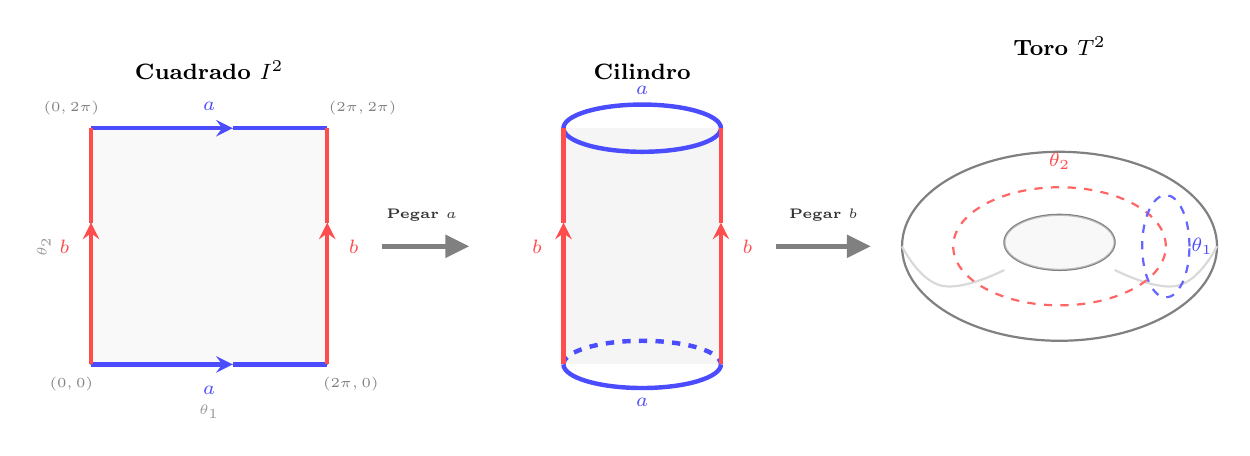
\begin{tikzpicture}[>=stealth, scale=1.0, every node/.style={font=\small}]

% =============================================
% PASO 1: Cuadrado unitario con identificaciones
% =============================================
\begin{scope}[shift={(-5.5,0)}]
    \node[anchor=south, font=\bfseries\footnotesize] at (1.5, 3.5) {Cuadrado $I^2$};
    
    % Cuadrado
    \fill[gray!5] (0,0) rectangle (3,3);
    \draw[black!40, thin] (0,0) rectangle (3,3);
    
    % Borde inferior (flecha a la derecha, azul)
    \draw[blue!70, ultra thick, ->] (0,0) -- (1.8,0);
    \draw[blue!70, ultra thick] (1.8,0) -- (3,0);
    \node[font=\scriptsize, blue!70, anchor=north] at (1.5,-0.15) {$a$};
    
    % Borde superior (flecha a la derecha, azul — mismo sentido = se pegan)
    \draw[blue!70, ultra thick, ->] (0,3) -- (1.8,3);
    \draw[blue!70, ultra thick] (1.8,3) -- (3,3);
    \node[font=\scriptsize, blue!70, anchor=south] at (1.5,3.1) {$a$};
    
    % Borde izquierdo (flecha hacia arriba, rojo)
    \draw[red!70, ultra thick, ->] (0,0) -- (0,1.8);
    \draw[red!70, ultra thick] (0,1.8) -- (0,3);
    \node[font=\scriptsize, red!70, anchor=east] at (-0.15,1.5) {$b$};
    
    % Borde derecho (flecha hacia arriba, rojo — mismo sentido = se pegan)
    \draw[red!70, ultra thick, ->] (3,0) -- (3,1.8);
    \draw[red!70, ultra thick] (3,1.8) -- (3,3);
    \node[font=\scriptsize, red!70, anchor=west] at (3.15,1.5) {$b$};
    
    % Etiquetas de esquinas
    \node[font=\tiny, black!50] at (-0.25,-0.25) {$(0,0)$};
    \node[font=\tiny, black!50] at (3.3,-0.25) {$(2\pi,0)$};
    \node[font=\tiny, black!50] at (-0.25,3.25) {$(0,2\pi)$};
    \node[font=\tiny, black!50] at (3.45,3.25) {$(2\pi,2\pi)$};
    
    % Ejes dentro del cuadrado
    \node[font=\tiny\bfseries, gray!80] at (1.5,-0.6) {$\theta_1$};
    \node[font=\tiny\bfseries, gray!80, rotate=90] at (-0.6,1.5) {$\theta_2$};
\end{scope}

% =============================================
% FLECHA: Paso 1 → Paso 2
% =============================================
\draw[ultra thick, black!50] (-1.8,1.5) -- (-0.9,1.5); % La línea termina un poco antes
\fill[black!50] (-0.7,1.5) -- (-1.0,1.65) -- (-1.0,1.35) -- cycle; % Dibujamos el triángulo
\node[anchor=south, font=\tiny\bfseries, black!80] at (-1.3,1.7) {Pegar $a$};

% =============================================
% PASO 2: Cilindro (bordes azules pegados)
% =============================================
\begin{scope}[shift={(0.5,0)}]
    \node[anchor=south, font=\bfseries\footnotesize] at (1, 3.5) {Cilindro};
    
    % Cuerpo del cilindro
    \fill[gray!8] (0,0) -- (2,0) -- (2,3) -- (0,3) -- cycle;
    
    % BORDE SUPERIOR (Borde 'a' pegado)
    % Lo dibujamos en azul ultra thick para indicar que es la unión de los bordes 'a'
    \draw[blue!70, ultra thick] (1,3) ellipse (1 and 0.3);
    \node[font=\scriptsize, blue!70, anchor=south] at (1,3.3) {$a$};
    
    % BORDE INFERIOR (Borde 'a' pegado)
    % Parte de atrás punteada, parte de adelante sólida y azul
    \draw[blue!70, ultra thick, dashed] (0,0) arc[start angle=180, end angle=0, x radius=1, y radius=0.3];
    \draw[blue!70, ultra thick] (0,0) arc[start angle=180, end angle=360, x radius=1, y radius=0.3];
    \node[font=\scriptsize, blue!70, anchor=north] at (1,-0.3) {$a$};
    
    % Lados del cilindro (Bordes 'b' rojos)
    \draw[red!70, ultra thick, ->] (0,0) -- (0,1.8);
    \draw[red!70, ultra thick] (0,1.8) -- (0,3);
    \node[font=\scriptsize, red!70, anchor=east] at (-0.15,1.5) {$b$};
    
    \draw[red!70, ultra thick, ->] (2,0) -- (2,1.8);
    \draw[red!70, ultra thick] (2,1.8) -- (2,3);
    \node[font=\scriptsize, red!70, anchor=west] at (2.15,1.5) {$b$};
\end{scope}
% =============================================
% FLECHA: Paso 2 → Paso 3
% =============================================
% 1. La línea (termina en 4.2 en lugar de 4.4 para dejar espacio al triángulo)
\draw[ultra thick, black!50] (3.2,1.5) -- (4.2,1.5);
% Coordenadas: (Punta), (Esquina superior atrás), (Esquina inferior atrás)
\fill[black!50] (4.4, 1.5) -- (4.1, 1.65) -- (4.1, 1.35) -- cycle;
\node[anchor=south, font=\tiny\bfseries, black!80] at (3.8,1.7) {Pegar $b$};

% =============================================
% PASO 3: Toro T² (dona)
% =============================================
\begin{scope}[shift={(6.8,1.5)}]
    \node[anchor=south, font=\bfseries\footnotesize] at (0, 2.3) {Toro $T^2$};
    
    % Toro exterior
    \draw[black!50, thick] (0,0) ellipse (2 and 1.2);
    
    % Agujero del toro
    \draw[black!50, thick] (0,0.05) ellipse (0.7 and 0.35);
    
    % Curvas de profundidad
    \draw[gray!30, thick] 
        plot[smooth, tension=0.8] coordinates {(-2,0) (-1.5,-0.5) (-0.7,-0.3)};
    \draw[gray!30, thick] 
        plot[smooth, tension=0.8] coordinates {(0.7,-0.3) (1.5,-0.5) (2,0)};
    
    \fill[gray!10, opacity=0.5] (0,0.05) ellipse (0.7 and 0.35);
    
    % --- EL CAMBIO ESTÁ AQUÍ ---
    
    % θ₂: Ahora es el círculo GRANDE (azul) que recorre la dona
    % Porque viene del eje vertical que se estiró al cerrar el cilindro
    \draw[red!60, thick, dashed] (0,0) ellipse (1.35 and 0.75);
    \node[font=\scriptsize, red!70, anchor=south] at (0,0.85) {$\theta_2$};
    
    % θ₁: Ahora es el círculo PEQUEÑO (azul) que es la sección del cilindro
    % Es el que se formó al "pegar a"
    \draw[blue!60, thick, dashed] (1.35,0) ellipse (0.3 and 0.65);
    \node[font=\scriptsize, blue!70, anchor=west] at (1.55,0) {$\theta_1$};
\end{scope}

\end{tikzpicture}


    \caption{Representación topológica de la construcción del Toro $T^2$ a partir del cuadrado unitario mediante la identificación de bordes.}
    \label{fig:construccion_toro}
\end{figure}

Para que este conjunto de $n$-tuplas posea una noción rigurosa de cercanía y 
continuidad, indispensable para la planificación de trayectorias, se le dota de 
la \textit{topología producto} \parencite{antonyan2016topologia}. Bajo este esquema, 
los conjuntos abiertos básicos de $T^n$ se definen mediante el producto 
cartesiano de subconjuntos abiertos de cada factor individual; si se elige un 
arco abierto $U_i$ en cada $i$-ésimo círculo $S^1$, el 
producto $U_1 \times U_2 \times \dots \times U_n$ forma un hiperrectángulo curvo. 
Matemáticamente, esta estructura es la topología más débil que garantiza que 
las proyecciones desde el espacio total hacia cada articulación 
individual ($\pi_i: T^n \to S^1$) sean funciones continuas y abiertas.

Finalmente, una propiedad crucial para la optimización es la compacidad del espacio, 
la cual asegura que algoritmos de búsqueda no diverjan al infinito. En la 
topología moderna, la compacidad del Toro se justifica de manera intrínseca 
mediante el \textit{Teorema de Tíconov} \parencite{waldmann2014topology}, evitando la 
dependencia restrictiva de incrustaciones euclidianas y el Teorema de Heine-Borel. 
Dado que el Teorema de Tíconov establece que el producto de espacios 
compactos es, en sí mismo, un espacio compacto \parencite{antonyan2016topologia}, y 
siendo $S^1$ inherentemente compacto, $T^n$ hereda esta propiedad de forma absoluta.

En la robótica topológica, esta compacidad garantiza que cualquier 
función continua sobre $T^n$, como una función de costo, un campo vectorial 
para navegación o las ecuaciones de cinemática directa, alcance siempre sus valores 
máximos y mínimos absolutos. Así, el manipulador opera en un espacio que, 
aunque carece de fronteras físicas al ser una variedad cerrada, constituye 
un entorno matemáticamente compacto, acotado y determinista.


% % - Topología cociente: La identificación de bordes (0 y 2\pi). 
% % - Formalización de T^n como el espacio natural del Brazo Robótico Comunitario.
Habiendo establecido estas propiedades topológicas fundamentales, 
es posible particularizar este marco abstracto al diseño del Brazo Robótico Comunitario. 
Este manipulador está constituido mecánicamente por una cadena cinemática de $n$ 
articulaciones de revolución. Dado que la operación del sistema requiere el 
monitoreo continuo de cada eje rotacional, el vector de estado articular 
$q = (q_1, q_2, \dots, q_n)$ habita de forma nativa en la variedad $T^n$.

Definir a $T^n$ 
como el espacio de configuraciones natural de este brazo comunitario presenta una clara ventaja 
operativa: permite que los algoritmos de control de bajo nivel hereden la topología del 
Toro para resolver automáticamente las discontinuidades angulares, garantizando la 
interpolación de trayectorias por el camino más corto incluso al cruzar el umbral de 
los $360^\circ$. No obstante, una desventaja teórica a considerar en la implementación 
física es la presencia de topes mecánicos o cableado limitante; si una articulación no 
puede girar libremente los $360^\circ$, su representación topológica se degrada de un 
círculo cerrado $S^1$ a un intervalo euclidiano simple, lo que matemáticamente equivale a 
realizar cortes en el Toro, alterando la compacidad y conectividad global de la variedad. 
A pesar de estas restricciones prácticas, el Toro se mantiene como la estructura topológica 
subyacente que modela la cinemática íntegra del manipulador.


\subsection{Métricas en variedades y topología métrica}
% - Definición de las métricas L_1 (Manhattan) y L_2 (Euclidiana).

Cuando trabajamos con variedades topológicas (como el espacio de configuraciones de un robot), 
a menudo resulta útil y necesario dotarlas de una función cuantitativa de distancia, 
convirtiéndolas formalmente en espacios métricos. 

Dado un espacio métrico $(X, d)$, la función de distancia $d$ induce de manera intrínseca una 
topología sobre $X$, denotada usualmente como $\tau_d$ e identificada como la \textit{topología 
métrica} \parencite{antonyan2016topologia}. En esta topología, los conjuntos abiertos básicos 
que estructuran el espacio se 
definen a partir de las bolas abiertas generadas por la métrica:

$$ B_r(x) = \{y \in X \mid d(x,y) < r\} $$

Cualquier subconjunto $O \subset X$ es abierto en esta topología si puede expresarse 
como una unión de dichas bolas abiertas \parencite{waldmann2014topology}.

Para modelar los entornos locales de una variedad (cartas que se mapean a $\mathbb{R}^n$), 
existen diversas formas de cuantificar la distancia entre dos puntos 
$x = (x_1, \dots, x_n)$ e $y = (y_1, \dots, y_n)$. Dos de las métricas más importantes 
y comúnmente implementadas en algoritmos computacionales y robótica son la métrica euclidiana 
y la métrica de Manhattan \parencite{antonyan2016topologia}.

\textbf{Métrica $L_1$ (Métrica de Manhattan):} En aplicaciones donde el movimiento no puede realizarse 
en línea recta diagonal, sino que está restringido a ejes ortogonales 
(como los desplazamientos en una retícula o un brazo cartesiano), se define la 
métrica $L_1$ o de Manhattan. Se define mediante la suma de las diferencias absolutas de cada 
coordenada:
$$ d_1(x, y) = \sum_{i=1}^n |x_i - y_i| $$
Geométricamente, esta métrica representa la distancia mínima que un vehículo tendría que 
recorrer moviéndose a través de una cuadrícula de calles para ir del punto $x$ al punto $y$.

\textbf{Métrica $L_2$ (Métrica Euclidiana):} Es la formulación matemática de la distancia 
geométrica en línea recta clásica. Se deriva directamente del producto interno (o punto) 
estándar en $\mathbb{R}^n$ y su norma asociada. Se define como:
$$ d_2(x, y) = \sqrt{\sum_{i=1}^n (x_i - y_i)^2} $$
Esta función cumple rigurosamente con los axiomas de un espacio métrico 
(positividad, simetría y desigualdad del triángulo). La topología generada por esta 
métrica en $\mathbb{R}^n$ recibe el nombre de \textit{topología euclidiana}.

Un concepto relevante en la topología métrica es que es posible definir más de una 
métrica sobre el mismo conjunto. Si se pueden encontrar constantes $m, M > 0$ tales que 
para cualquier par de puntos se cumpla $m \cdot d_1(x,y) \le d_2(x,y) \le M \cdot d_1(x,y)$, 
entonces ambas métricas se consideran métricamente equivalentes \parencite{waldmann2014topology}. 

En el espacio $\mathbb{R}^n$, las métricas $L_1$ y $L_2$ (junto con otras como la métrica 
del supremo $L_\infty$) arrojan valores numéricos distintos para la distancia, 
pero son topológicamente equivalentes \parencite{manetti2023topology}. Esto significa 
que, sin importar cuál de ellas elija 
el algoritmo del robot para calcular una ruta, ambas generarán exactamente la misma 
familia de conjuntos abiertos y, por tanto, idénticas nociones de vecindad, límite y continuidad.

Sin embargo, la aplicación directa de estas métricas sobre las coordenadas angulares 
crudas del manipulador (tratadas como vectores en $\mathbb{R}^n$) ignora la topología 
cíclica del espacio $T^n$. Para calcular la verdadera distancia geodésica (el camino más corto 
sobre la superficie de la variedad) es necesario adaptar estas funciones utilizando la 
aritmética modular inducida por la topología cociente.

Para un par de ángulos $\theta_1, \theta_2 \in S^1$, la distancia geodésica se define 
como el mínimo arco posible entre ellos:
$$ d_{S^1}(\theta_1, \theta_2) = \min(|\theta_1 - \theta_2|, 2\pi - |\theta_1 - \theta_2|) $$

Esta definición, conocida computacionalmente como distancia \textit{wrap-around} \parencite{lynch2017modern}, permite 
que el algoritmo evalúe correctamente que la distancia entre 
$359^\circ$ y $1^\circ$ es de $2^\circ$ y no de $358^\circ$. Extendiendo este concepto al 
Toro $T^n$, la métrica global se construye aplicando esta corrección a 
cada componente articular antes de operar con la norma $L_1$ o $L_2$.


\section{Geometría del espacio de estados y conectividad}
% NOTA DE ESTRATEGIA: En esta sección traducimos el hardware del TESH a la matemática de la UnADM. 
% Aquí entra tu aportación principal: las bolas abiertas y las inestabilidades.

Una vez establecidos los fundamentos topológicos abstractos y la estructura métrica del Toro, 
es imperativo vincular este formalismo con la realidad operativa del manipulador robótico. 
En esta sección se aborda la transición del entorno físico, gobernado por dimensiones y 
obstáculos euclidianos, hacia su representación analítica como un espacio de estados. Al 
mapear los volúmenes de colisión y aplicar la teoría de recubrimientos mediante uniones de 
bolas abiertas, se delimita matemáticamente el subespacio seguro en el cual el robot puede 
navegar. Este análisis geométrico culmina en el estudio de la conectividad por caminos, un 
principio que determina de forma absoluta si una ruta entre dos configuraciones es 
viable antes de que cualquier algoritmo intente calcularla.



\subsection{Mapeo del espacio de trabajo al espacio de configuración ($\mathcal{C}$-Space)}
% - Definición formal del espacio libre (\mathcal{C}_{free}) y la región de obstáculos (\mathcal{C}_{obs}).

Para que un manipulador interactúe con su entorno, es necesario vincular 
matemáticamente su estado articular interno con la posición espacial de su efector 
final. En robótica, al conjunto de todas las posiciones y orientaciones alcanzables 
se le denomina \textit{espacio de trabajo} $\mathcal{W}$ (o \textit{task space}) \parencite{lynch2017modern}.

La relación entre el espacio de configuración $\mathcal{C}$ y el espacio de 
trabajo $\mathcal{W}$ está gobernada por una aplicación continua 
$F: \mathcal{C} \to \mathcal{W}$, conocida como mapa 
cinemático directo \parencite{grant2015topology}. Esta función asocia, 
de manera determinista, cada configuración articular con las coordenadas 
exactas del extremo del robot en el espacio euclidiano \parencite{grant2015topology}.

En escenarios de aplicación real, $\mathcal{W}$ suele estar limitado por 
restricciones físicas u objetos externos. Dado que los algoritmos de control 
planifican rutas en el espacio topológico $\mathcal{C}$ y no directamente en el 
entorno euclidiano $\mathcal{W}$ \parencite{grant2015topology}, es necesario 
mapear estas restricciones. Para ello, se define formalmente 
la \textit{región de obstáculos} $\mathcal{C}_{obs}$ como el 
conjunto de configuraciones $q \in \mathcal{C}$ en las cuales el 
volumen ocupado por los eslabones del robot colisiona con algún objeto del 
entorno \parencite{lynch2017modern}. En sistemas multi-robot o 
mecanismos propensos a auto-intersecciones, esto se generaliza mediante 
la \enquote{diagonal de colisión} $\Delta$, que agrupa las configuraciones donde dos 
partes físicas intentan ocupar la misma coordenada 
simultáneamente \parencite{oniani2019topology}.

Para garantizar movimientos físicamente realizables, el algoritmo de planificación 
se restringe a las áreas sin interferencias. Esto da 
lugar al \textit{espacio libre} $\mathcal{C}_{free}$ (también denominado $SC$ 
por \textit{safe configuration space}), definido como 
la sustracción de la región de obstáculos respecto al espacio 
total \parencite{oniani2019topology}:

$$ \mathcal{C}_{free} = \mathcal{C} \setminus \mathcal{C}_{obs} $$

\begin{figure}[htbp]
    \centering
    % !TeX root = ../main.tex
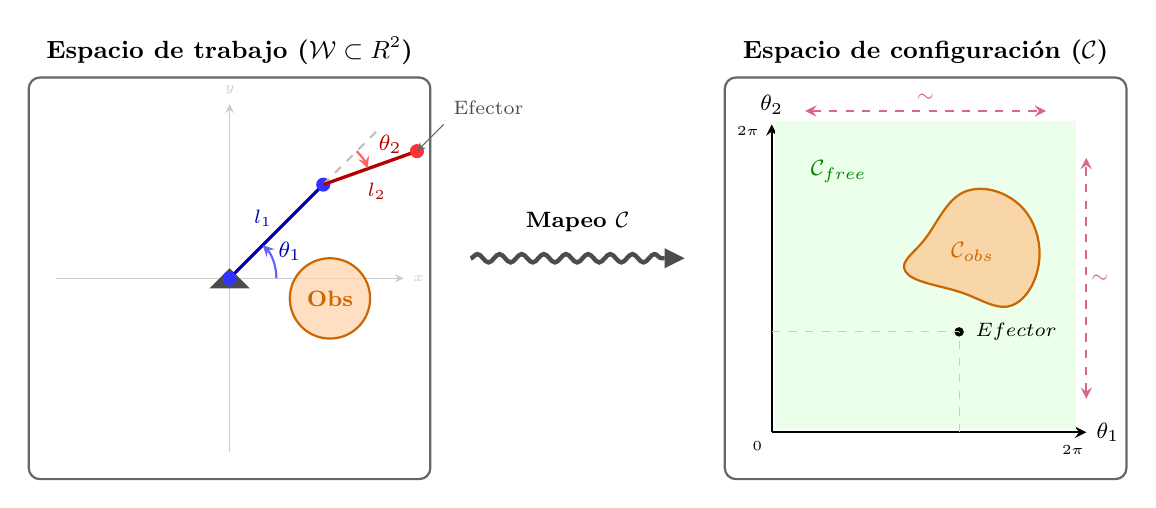
\begin{tikzpicture}[>=stealth, scale=0.85, every node/.style={font=\small}]

% =============================================
% PANEL IZQUIERDO: Espacio de Trabajo (W)
% =============================================
\begin{scope}[shift={(-5.2,0)}]
    \node[anchor=south, font=\bfseries\small] at (0, 3.05) {Espacio de trabajo ($\mathcal{W} \subset \mathbb{R}^2$)};
    \draw[rounded corners=4pt, thick, black!60] (-3.0,-3.0) rectangle (3.0,3.0);
    
    % Ejes
    \draw[->, gray!40] (-2.6,0) -- (2.6,0) node[right, font=\tiny] {$x$};
    \draw[->, gray!40] (0,-2.6) -- (0,2.6) node[above, font=\tiny] {$y$};
    
    % Base
    \fill[black!70] (-0.3,-0.15) -- (0.3,-0.15) -- (0,0.15) -- cycle;
    
    % Articulaciones (Coordenadas directas)
    \coordinate (J0) at (0,0);
    \coordinate (J1) at (1.4,1.4); % l1 a 45 grados aprox
    \coordinate (J2) at (2.8,1.9); % l2 inclinado
    
    % --- Brazo 1 ---
    \draw[very thick, blue!70!black] (J0) -- (J1);
    \fill[blue!80] (J0) circle (3pt);
    \fill[blue!80] (J1) circle (3pt);
    \node[blue!70!black, font=\scriptsize] at (0.5,0.9) {$l_1$};
    
    % Arco theta 1
    \draw[->, blue!60, thick] (0.7,0) arc (0:45:0.7);
    \node[blue!70!black, font=\footnotesize] at (0.9,0.4) {$\theta_1$};
    
    % --- Referencia Punteada (Extensión de l1) ---
    \draw[gray!50, thick, dashed] (J1) -- (2.2,2.2);
    
    % --- Brazo 2 ---
    \draw[very thick, red!70!black] (J1) -- (J2);
    \fill[red!80] (J2) circle (3pt);
    \node[red!70!black, font=\scriptsize] at (2.2,1.3) {$l_2$};
    
    % Arco theta 2 (basado en la extensión de l1)
    \draw[->, red!60, thick] (1.9,1.9) arc (45:20:0.7);
    \node[red!70!black, font=\footnotesize] at (2.4,2) {$\theta_2$};
    
    % Efector
    \draw[<-, thin, black!60] (J2) -- ++(0.4, 0.4);
    \node[font=\scriptsize, anchor=south west, black!70] at (3.2,2.3) {Efector};
    
    % Obstáculo
    \fill[orange!35, opacity=0.7] (1.5, -0.3) circle (0.6);
    \draw[orange!80!black, thick] (1.5, -0.3) circle (0.6);
    \node[font=\footnotesize\bfseries, orange!80!black] at (1.5, -0.3) {Obs};
\end{scope}

% =============================================
% FLECHA CENTRAL
% =============================================
\draw[ultra thick, black!70, decorate, decoration={snake, amplitude=1.5pt, segment length=8pt, post length=1pt}] (-1.6,0.3) -- (1.3,0.3);
\fill[black!70] (1.6, 0.3) -- (1.3, 0.45) -- (1.3, 0.15) -- cycle;
\node[anchor=south, font=\footnotesize\bfseries] at (0,0.55) {Mapeo $\mathcal{C}$};

% =============================================
% PANEL DERECHO: Espacio de Configuración (C)
% =============================================
\begin{scope}[shift={(5.2,0)}]
    \node[anchor=south, font=\bfseries\small] at (0, 3.05) {Espacio de configuración ($\mathcal{C}$)};
    \draw[rounded corners=4pt, thick, black!60] (-3.0,-3.0) rectangle (3.0,3.0);
    
    % Ejes movidos ligeramente para no chocar con el marco
    \draw[->, thick] (-2.3,-2.3) -- (2.4,-2.3) node[right, font=\footnotesize] {$\theta_1$};
    \draw[->, thick] (-2.3,-2.3) -- (-2.3,2.3) node[above, font=\footnotesize] {$\theta_2$};
    
    \node[font=\tiny, anchor=north east] at (-2.3,-2.3) {$0$};
    \node[font=\tiny, anchor=north] at (2.2,-2.35) {$2\pi$};
    \node[font=\tiny, anchor=east] at (-2.35,2.2) {$2\pi$};
    
    \fill[green!8] (-2.25,-2.25) rectangle (2.25,2.35);
    
    \fill[orange!45, opacity=0.7] 
        plot[smooth cycle, tension=0.7] 
        coordinates {(0.0,0.6) (0.6,1.3) (1.4,1.1) (1.7,0.3) (1.3,-0.4) (0.5,-0.2) (-0.3,0.1)};
    \draw[orange!80!black, thick] 
        plot[smooth cycle, tension=0.7] 
        coordinates {(0.0,0.6) (0.6,1.3) (1.4,1.1) (1.7,0.3) (1.3,-0.4) (0.5,-0.2) (-0.3,0.1)};
    
    % Etiquetas reposicionadas para visibilidad
    \node[font=\footnotesize\bfseries, orange!80!black] at (0.7,0.4) {$\mathcal{C}_{obs}$};
    \node[font=\footnotesize, green!50!black] at (-1.3,1.6) {$\mathcal{C}_{free}$};
    
    % Topología (Simetría)
    \draw[<->, dashed, purple!60, thick] (2.4,-1.8) -- (2.4,1.8);
    \node[font=\scriptsize, purple!60] at (2.6,0.0) {$\sim$};
    
    \draw[<->, dashed, purple!60, thick] (-1.8,2.5) -- (1.8,2.5);
    \node[font=\scriptsize, purple!60] at (0.0,2.7) {$\sim$};

    % --- PUNTO DE CONFIGURACIÓN ACTUAL ---
    % Elegimos una coordenada que coincida visualmente con el dibujo del brazo (ej. θ1=45°, θ2=20°)
    % En escala del C-space de -2.3 a 2.3, esto sería aprox (0.5, -0.8) 
    \fill[black] (0.5, -0.8) circle (2pt);
    \node[anchor=west, font=\scriptsize] at (0.6, -0.8) {$Efector$};
    
    % Opcional: Líneas de proyección a los ejes para mayor claridad
    \draw[gray!40, dashed, thin] (0.5, -2.3) -- (0.5, -0.8);
    \draw[gray!40, dashed, thin] (-2.3, -0.8) -- (0.5, -0.8);

\end{scope}

\end{tikzpicture}

    \caption{Mapeo de un obstáculo desde el espacio de trabajo euclidiano ($\mathcal{W}$) hacia la región prohibida ($\mathcal{C}_{obs}$) en el espacio de configuración.}
    \label{fig:mapeo_cspace}
\end{figure}

Como se observa en la Figura \ref{fig:mapeo_cspace}, para un manipulador articulado de $n$ grados de revolución operando en el 
espacio euclidiano tridimensional ($\mathcal{W} \subset \mathbb{R}^3$), 
el espacio de configuración es el toro $T^n$. La introducción de un 
obstáculo físico (como una caja sólida en $\mathbb{R}^3$) no 
resulta en un simple bloqueo geométrico, sino en una \textit{restricción topológica}. 
A través del mapeo cinemático inverso, el volumen del obstáculo 
se transforma en una región prohibida multidimensional sobre la superficie de $T^n$.

Topológicamente, sustraer $\mathcal{C}_{obs}$ equivale a \enquote{perforar} el toro original. 
Dependiendo de la ubicación y tamaño del obstáculo en $\mathbb{R}^3$, su 
preimagen puede separar $T^n$ en componentes disconexas o crear \enquote{agujeros} que alteran 
fundamentalmente sus propiedades homotópicas y su grupo fundamental 
\parencite{Mosquera2017}. Esta transición justifica el uso de la topología: 
el algoritmo ya no calcula distancias euclidianas a una caja, sino que resuelve 
el problema de deformar una curva alrededor de los agujeros en la variedad 
perforada $T^n \setminus \mathcal{C}_{obs}$ \parencite{farber2008}.

Gracias a esta formulación, la evasión de colisiones se reduce a encontrar una 
trayectoria continua $p: [0, 1] \to \mathcal{C}_{free}$ \parencite{Mosquera2017} 
que conecte dos configuraciones seguras, evitando por completo el conjunto 
prohibido $\mathcal{C}_{obs}$ \parencite{lynch2017modern}. En última instancia, 
son la compacidad, la conexidad y las propiedades métricas de $\mathcal{C}_{free}$ 
las que determinan si el objetivo es alcanzable o si el robot carece de una ruta 
libre \parencite{oniani2019topology}.


\subsection{Teoría de recubrimientos y aproximación por bolas abiertas}
% % - Sustento topológico para la detección de colisiones: uso de familias de conjuntos abiertos (bolas) para recubrir el volumen del manipulador.
% % - Justificación de cómo este modelo matemático optimiza el cálculo frente a métodos tradicionales de ingeniería (cajas AABB), manteniendo la consistencia topológica.

En el modelado físico, el volumen ocupado por cada eslabón de un 
manipulador robótico constituye un subconjunto cerrado y acotado en 
el espacio euclidiano $\mathbb{R}^3$. Por el Teorema de Heine-Borel, 
este volumen se caracteriza como un espacio topológico compacto \parencite{antonyan2016topologia}. Una propiedad 
fundamental de los espacios métricos compactos es que son 
totalmente acotados, lo que implica que para cualquier radio 
$\epsilon > 0$, el espacio puede ser recubierto íntegramente 
mediante una familia finita de bolas abiertas 
$B(p_i, \epsilon)$ \parencite{antonyan2016topologia}.

Esta propiedad constituye la base matemática de la 
\textit{aproximación esférica de la geometría del robot} 
\parencite{coumar2025foam}. En lugar de evaluar colisiones sobre 
la compleja topología de las mallas poligonales 
originales, las cuales frecuentemente presentan defectos geométricos 
o no constituyen variedades estancas (\textit{watertight}), 
el volumen del robot se aproxima mediante un recubrimiento finito de 
primitivas esféricas \parencite{coumar2025foam}. Algoritmos como la 
aproximación adaptativa del eje medial (AMAA) emplean este principio 
para encajar un conjunto finito de bolas en el interior de la malla. De 
este modo, la geometría física se simplifica a una unión finita de 
conjuntos abiertos básicos generados por la métrica del espacio 
\parencite{coumar2025foam}.

Tradicionalmente, la ingeniería ha abordado la detección de colisiones 
envolviendo la geometría en volúmenes delimitadores poliédricos, 
como las cajas alineadas con los ejes 
(AABB, \textit{Axis-Aligned Bounding Boxes}) o descomposiciones en 
cuboides \parencite{coumar2025foam}. Sin embargo, calcular 
la distancia mínima entre un punto y un poliedro es un proceso 
algebraicamente costoso, pues requiere evaluar múltiples caras, aristas y 
vértices en función de la orientación espacial. La Figura \ref{fig:bolas_vs_aabb} 
contrasta visualmente esta aproximación tradicional frente al recubrimiento topológico.

\begin{figure}[htbp]
    \centering
    % !TeX root = ../main.tex
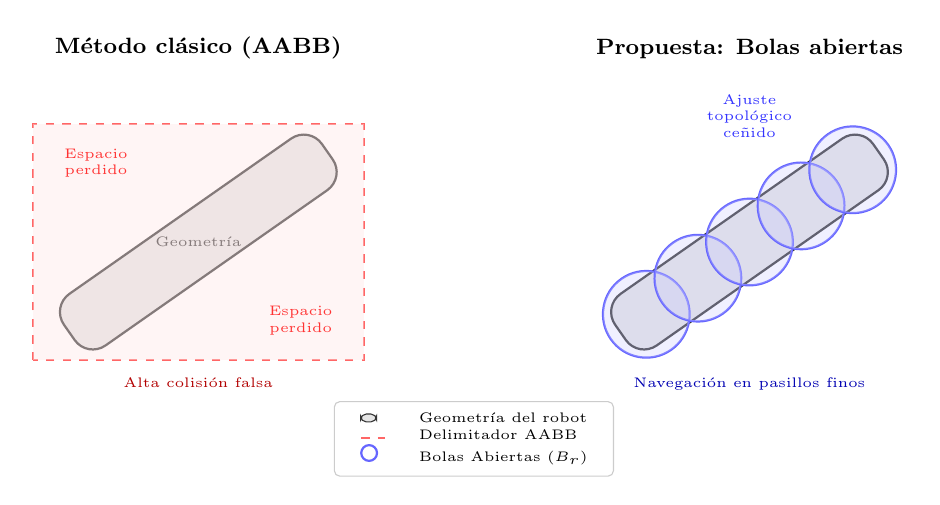
\begin{tikzpicture}[>=stealth, scale=1.0, every node/.style={font=\small}]

% Estilo para el eslabón del robot (geometría original)
\tikzset{
    robotlink/.style={
        draw=black!80, 
        fill=gray!20, 
        rounded corners=8pt, 
        thick
    }
}

% =============================================
% PANEL IZQUIERDO: Bounding Box Clásica (AABB)
% =============================================
\begin{scope}[shift={(-3.5,0)}]
    \node[anchor=south, font=\bfseries\footnotesize] at (0, 2.2) {Método clásico (AABB)};
    
    % Dibujamos el eslabón inclinado
    \begin{scope}[rotate=35]
        \draw[robotlink] (-2, -0.4) rectangle (2, 0.4);
        \node[font=\tiny, black!80] at (0,0) {Geometría};
    \end{scope}

    % Caja AABB (Rectángulo ortogonal que lo encierra)
    % El brazo rotado 35 grados tiene una caja que lo encierra de aprox 4x3
    \draw[red!60, dashed, thick] (-2.1, -1.5) rectangle (2.1, 1.5);
    \fill[red!10, opacity=0.4] (-2.1, -1.5) rectangle (2.1, 1.5);
    
    % Etiquetas de ineficiencia
    \node[red!80, font=\tiny, text width=1.5cm, align=center] at (-1.3, 1.0) {Espacio perdido};
    \node[red!80, font=\tiny, text width=1.5cm, align=center] at (1.3, -1.0) {Espacio perdido};
    
    \node[anchor=north, font=\tiny, text=red!70!black] at (0, -1.6) {Alta colisión falsa};
\end{scope}

% =============================================
% PANEL DERECHO: Bolas Abiertas (Propuesta)
% =============================================
\begin{scope}[shift={(3.5,0)}]
    \node[anchor=south, font=\bfseries\footnotesize] at (0, 2.2) {Propuesta: Bolas abiertas};
    
    % Dibujamos el eslabón inclinado (mismo ángulo)
    \begin{scope}[rotate=35]
        \draw[robotlink] (-2, -0.4) rectangle (2, 0.4);
    \end{scope}

    % Recubrimiento por bolas (cadena de esferas)
    \begin{scope}[rotate=35]
        \foreach \x in {-1.6, -0.8, 0, 0.8, 1.6} {
            \draw[blue!60, thick] (\x, 0) circle (0.55);
            \fill[blue!20, opacity=0.3] (\x, 0) circle (0.55);
        }
    \end{scope}
    
    % Etiquetas de eficiencia
    \node[blue!80, font=\tiny, text width=1.8cm, align=center] at (0, 1.6) {Ajuste topológico ceñido};
    
    \node[anchor=north, font=\tiny, text=blue!70!black] at (0, -1.6) {Navegación en pasillos finos};
\end{scope}

% =============================================
% LEYENDA CENTRAL
% =============================================
\node[draw=black!20, rounded corners=2pt, fill=white, font=\tiny] at (0,-2.5) {
    \begin{tabular}{ll}
    \tikz\fill[gray!20, draw=black!80] (0,0) rectangle (0.2,0.1); & Geometría del robot \\
    \tikz\draw[red!60, dashed, thick] (0,0) -- (0.3,0); & Delimitador AABB \\
    \tikz\draw[blue!60, thick] (0,0) circle (0.1); & Bolas Abiertas ($B_r$)
    \end{tabular}
};

\end{tikzpicture}

    \caption{Comparativa geométrica entre el delimitador clásico por cajas ortogonales (AABB) y el recubrimiento topológico mediante uniones finitas de bolas abiertas.}
    \label{fig:bolas_vs_aabb}
\end{figure}

El modelo topológico basado en recubrimientos por bolas abiertas 
optimiza drásticamente este cálculo. A diferencia de los poliedros, 
cuyas aristas introducen discontinuidades, las esferas facilitan la 
evaluación de funciones continuas críticas, como los Campos de 
Distancia Signada (SDF) y las Transformadas de Distancia Euclidiana 
(EDT), esenciales para los métodos modernos de optimización de 
gradiente \parencite{coumar2025foam}. 

Bajo este enfoque, el cálculo de colisiones se reduce a evaluar la 
métrica euclidiana $L_2$ entre el centro geométrico de la bola y el 
obstáculo, restando simplemente el radio de la primitiva 
\parencite{coumar2025foam}. La literatura demuestra que estas 
aproximaciones aceleran las consultas de distancia hasta en dos 
órdenes de magnitud en comparación con los modelos tradicionales 
\parencite{coumar2025foam}. 

Finalmente, este método asegura una estricta consistencia topológica. 
Al generar el recubrimiento, es posible controlar el nivel de fidelidad 
para garantizar una sobreaproximación conservadora del volumen real 
\parencite{coumar2025foam}. Esto certifica que el espacio libre 
resultante ($\mathcal{C}_{free}$) sea topológicamente seguro: 
si el algoritmo identifica una trayectoria continua para el 
recubrimiento de bolas, se garantiza matemáticamente la ausencia 
de colisiones para el robot físico.


% \subsubsection{Conectividad por caminos e inestabilidades topológicas}
% % - Definición de camino continuo y componentes conexas en \mathcal{C}_{free}.
% % - El problema de los espacios no contráctiles (basado en Mosquera Lois y Farber): 
% % explicar por qué no existen algoritmos globales estables y cómo esto genera "saltos" o inestabilidades si no se planifica adecuadamente.

\subsection{Conectividad por caminos e inestabilidades topológicas}

Habiendo garantizado la consistencia topológica del espacio libre $\mathcal{C}_{free}$ mediante su recubrimiento, 
el problema de planificación de movimientos se reduce a encontrar 
rutas viables dentro de esta variedad. Matemáticamente, un movimiento 
o reubicación del robot desde una configuración inicial $A$ hasta 
una configuración final $B$ se define como un camino continuo 
(o trayectoria): una función continua \parencite{Mosquera2017} $\gamma: [0, 1] \to \mathcal{C}_{free}$ 
tal que $\gamma(0) = A$ y $\gamma(1) = B$ \parencite{antonyan2016topologia}.

Para que una configuración $B$ sea físicamente alcanzable desde $A$, 
ambas deben pertenecer a la misma componente conexa por caminos del 
espacio $\mathcal{C}_{free}$ \parencite{oniani2019topology}. La presencia de múltiples obstáculos 
tridimensionales puede fragmentar el espacio libre en diversas 
componentes disconexas. Si esto ocurre, no existirá ninguna trayectoria 
continua que una un punto de una componente con otro de una distinta 
sin atravesar la región prohibida $\mathcal{C}_{obs}$ \parencite{manetti2023topology}. Por lo tanto, 
un robot es \enquote{libremente transportable} a lo largo de todo el entorno 
si y solo si el espacio $\mathcal{C}_{free}$ en su totalidad es conexo 
por caminos \parencite{oniani2019topology}.


Incluso si el espacio de configuraciones es conexo por caminos, 
el diseño de un algoritmo de control global se enfrenta a un obstáculo 
topológico fundamental. Un algoritmo de planificación de movimientos 
se formaliza como una sección $s: X \times X \to PX$, donde $PX$ es 
el espacio de todos los caminos continuos y la función devuelve una 
ruta específica para cada par de estados inicial y final $(A, B)$ \parencite{Mosquera2017}. 
Idealmente, se desea que este algoritmo sea continuo (estable); es decir, 
que si los objetivos o las posiciones iniciales varían ligeramente, 
la ruta generada por el algoritmo varíe de forma igualmente sutil y 
predecible \parencite{Mosquera2017}.

Sin embargo, como demuestran Mosquera Lois y M. Farber, un algoritmo de 
planificación de movimientos global y continuo existe si y solo si el 
espacio de configuraciones es contráctil (es decir, puede deformarse de 
manera continua hasta un solo punto) \parencite{Mosquera2017, farber2008}. 

El problema radica en que los espacios de configuración 
robóticos (como la circunferencia $S^1$ para una articulación, 
el Toro $T^n$ para brazos múltiples, o $SO(3)$ para orientaciones) 
no son espacios contráctiles \parencite{Mosquera2017}. Como consecuencia directa del teorema 
de Farber, no existe ningún algoritmo global estable para el control 
de estos mecanismos \parencite{Mosquera2017}. Cualquier algoritmo informático que opere sobre 
todo el espacio de configuraciones presentará obligatoriamente puntos 
de discontinuidad \parencite{farber2008}.

La falta de continuidad en el algoritmo genera inestabilidades topológicas. 
Si no se planifica adecuadamente dividiendo el 
espacio en zonas seguras, la discontinuidad provocará que, 
para dos pares de estados $(A, B)$ y $(A', B')$ que están 
arbitrariamente cerca el uno del otro, el algoritmo devuelva 
rutas de movimiento diametralmente distintas \parencite{Mosquera2017}. 

Un ejemplo clásico ocurre en una simple articulación rotatoria 
($S^1$): si el robot debe ir del ángulo 
$0^\circ$ al $180^\circ$, el algoritmo debe \enquote{decidir} si girar en 
sentido horario o antihorario \parencite{Mosquera2017}. Una mínima perturbación en el destino 
(por ejemplo, moverse a $179.9^\circ$ en lugar de $180.1^\circ$) 
obligará a un algoritmo mal diseñado a dar un \enquote{salto} abrupto, 
invirtiendo de golpe el sentido de rotación y produciendo 
trayectorias completamente diferentes para escenarios casi 
idénticos \parencite{Mosquera2017}. Para mitigar esto, la robótica topológica se vale de la 
Complejidad Topológica ($TC$), fragmentando el espacio total 
mediante un recubrimiento finito de \enquote{abiertos de Farber} sobre 
los cuales sí es posible definir reglas de movimiento locales 
continuas e ininterrumpidas \parencite{Mosquera2017}.

\section{Planificación de trayectorias y arquitectura algorítmica en ROS2}
% NOTA DE ESTRATEGIA: Aquí justificamos el entorno de software.
% Explicamos cómo la teoría continua se vuelve discreta y se estructura dentro de un paquete "custom" 
% en ROS2, prescindiendo de planificadores de caja negra como MoveIt.

Una vez que el espacio de configuraciones ha sido rigurosamente definido como una variedad topológica 
y se han establecido las condiciones de conectividad, el siguiente paso es traducir este modelo 
abstracto en un problema resoluble computacionalmente. La teoría de variedades continuas, si bien 
es analíticamente poderosa, resulta intratable para un procesador digital, que opera sobre secuencias 
finitas de instrucciones. Por lo tanto, esta sección aborda la transición fundamental desde el 
continuo matemático hacia la estructura discreta de un grafo, un paso indispensable para la 
implementación de algoritmos de búsqueda.

Se explorarán dos paradigmas algorítmicos contrastantes para navegar este grafo. Primero, se 
analizará la búsqueda determinista mediante el algoritmo A*, examinando cómo la elección de una 
métrica y la estructura de la retícula toroidal impactan en la optimalidad de la solución. A 
continuación, se abordará la búsqueda estocástica con el algoritmo RRT, un método diseñado para 
sortear la \enquote{maldición de la dimensionalidad} mediante un muestreo probabilístico.

Finalmente, para materializar y validar estos conceptos, se detallará la arquitectura de software 
sobre la cual se implementarán. Se justifica el uso de un paquete personalizado dentro del ecosistema 
de ROS2, prescindiendo deliberadamente de planificadores de alto nivel como MoveIt. Este enfoque de 
\enquote{caja blanca} permite no solo ejecutar los algoritmos, sino también visualizar y analizar su 
comportamiento interno, conectando directamente la teoría topológica con la evidencia empírica.

\subsection{Discretización de la variedad y grafos métricos}
% - Explicar el paso matemático de un espacio continuo (T^n) a una partición discreta (retícula/grafo) manejable numéricamente.

En términos prácticos, el espacio de configuraciones de un mecanismo articulado, 
como la variedad topológica continua $T^n$, contiene una infinidad no numerable 
de estados. Dado que un procesador solo puede ejecutar una secuencia 
finita de instrucciones, resulta matemáticamente imposible evaluar de forma 
directa toda la variedad. Por lo tanto, para automatizar la planificación 
de movimiento, este espacio continuo debe reducirse a una estructura discreta, 
típicamente un grafo o una retícula de búsqueda \parencite{lavalle2006planning}.

La transición de la abstracción topológica hacia un modelo procesable 
computacionalmente se logra extrayendo una cantidad finita de puntos o 
\enquote{muestras} y estableciendo relaciones de adyacencia entre ellos. 
Este proceso se materializa principalmente mediante dos enfoques \parencite{lavalle2006planning}:

\begin{itemize}
\item \textbf{Retículas de búsqueda para algoritmos deterministas:} El método más 
directo consiste en superponer una cuadrícula o retícula (\textit{grid/lattice}) 
sobre la variedad continua $\mathcal{C}$. Computacionalmente, el espacio topológico 
se parametriza (por ejemplo, el hipercubo unitario $I^n$ con identificaciones en 
sus extremos para formar el Toro $T^n$ \parencite{Mosquera2017}) y se discretiza 
determinando una resolución o tamaño de paso para cada eje de coordenadas. 
A continuación, se define matemáticamente una \enquote{vecindad} (como la 
1-vecindad o 2-vecindad) que establece qué puntos de la retícula están conectados 
mediante aristas. El resultado es un grafo topológico regular sobre el cual los 
algoritmos deterministas (como A*) pueden operar para encontrar rutas 
óptimas \parencite{lavalle2006planning}.

\item \textbf{Grafos de muestreo para algoritmos estocásticos:} En configuraciones 
de alta dimensionalidad (alto $n$), las retículas regulares sufren de un 
crecimiento exponencial en la cantidad de nodos, lo que vuelve la búsqueda 
impracticable \parencite{choset2005principles}. Para solucionar este inconveniente, 
los algoritmos basados en muestreo 
abandonan la estructura de retícula y construyen incrementalmente un árbol 
o grafo unidimensional, explorando el espacio de forma probabilística o 
cuasialeatoria \parencite{lavalle2006planning}. Se genera una secuencia densa de muestras en el 
espacio libre, y un método de planificación local (LPM) traza aristas 
continuas y simples entre configuraciones cercanas. En el caso de los 
algoritmos RRT, por ejemplo, el árbol se expande estocásticamente 
buscando siempre conectarse con la muestra más cercana generada, 
logrando llenar el espacio de forma eficiente sin representarlo de 
manera exhaustiva \parencite{lavalle2006planning}.
\end{itemize}

Al realizar esta discretización, se asume una pérdida inherente y 
deliberada de la resolución geométrica. En el modelo continuo original, 
los límites de los obstáculos y la variedad libre $\mathcal{C}_{free}$ 
son exactos. Sin embargo, al discretizar el espacio, el grafo solo 
captura la conectividad de forma aproximada: el algoritmo \enquote{ciegamente} 
asume que el espacio entre los nodos de la retícula o 
las muestras del árbol se comporta de manera lineal o predecible \parencite{choset2005principles}. Si la 
resolución seleccionada es demasiado baja, el algoritmo fallará en 
detectar pasajes estrechos entre obstáculos y 
podría no encontrar una solución válida que matemáticamente sí existe \parencite{lavalle2006planning}. 

A pesar de esta pérdida geométrica, el sacrificio está plenamente 
justificado por la inmensa ganancia en eficiencia computacional \parencite{choset2005principles}. 
Mientras que los algoritmos combinatorios o geométricos \enquote{exactos} evalúan 
de forma analítica toda la topología de la variedad, se vuelven 
computacionalmente intratables a medida que crece la dimensionalidad 
del robot \parencite{lavalle2006planning}. Al reducir la variedad topológica a un grafo finito, 
los métodos basados en retículas o muestreo renuncian a la 
\enquote{completitud} matemática absoluta para alcanzar, en su lugar, una completitud por 
resolución o probabilística \parencite{choset2005principles}. Esto significa que transforman 
un problema geométrico irresoluble en un problema de búsqueda 
discreta que produce trayectorias seguras en un tiempo computacionalmente 
eficiente, bastando con refinar el nivel de muestreo 
(por ejemplo, añadiendo más nodos al grafo) en caso de que el algoritmo falle 
en su búsqueda inicial.


\subsection{Búsqueda determinista: Algoritmo A* en espacios no euclidianos}
% % - Fundamentos del algoritmo y el papel matemático de la heurística.
% % - Impacto de la selección métrica (L_1 vs L_2) en la convergencia dentro de la retícula toroidal.

Para planificar el movimiento sobre el grafo discretizado del espacio de configuraciones, 
el algoritmo de búsqueda A* determina sistemáticamente qué estado explorar a continuación 
mediante la evaluación de la función $f(n) = g(n) + h(n)$. En esta formulación, $g(n)$ 
representa el costo real acumulado desde el estado inicial hasta el nodo $n$, mientras que 
$h(n)$ es una función heurística que estima el costo del camino más corto desde $n$ hasta 
el objetivo \parencite{choset2005principles}.

El funcionamiento sistemático del algoritmo A* se rige por el siguiente algoritmo:

\vspace{0.3cm}
\noindent\textbf{Algoritmo: Búsqueda Determinista A* en Variedad Toroidal}
\begin{description}
    \item[\textbf{Entradas:}] Nodo inicial $q_{start} \in T^n$, Nodo objetivo $q_{goal} \in T^n$, Retícula topológica discretizada.
    \item[\textbf{Salida:}] Trayectoria óptima desde $q_{start}$ hasta $q_{goal}$.
    
    \item[\textbf{Paso 1 (Inicialización):}] Se añaden el nodo inicial $q_{start}$ a una \textit{Lista Abierta} vacía y se establece $g(q_{start}) = 0$. Se inicializa una \textit{Lista Cerrada}.
    
    \item[\textbf{Paso 2 (Iteración):}] Mientras la \textit{Lista Abierta} no esté vacía:
    \begin{enumerate}
        \item Se extrae el nodo $n$ de la \textit{Lista Abierta} que minimice $f(n) = g(n) + h(n)$.
        \item \textbf{Condición de Paro:} Si $n$ coincide con $q_{goal}$, se reconstruye y devuelve la trayectoria.
        \item Se remueve $n$ de la \textit{Lista Abierta} y se inserta en la \textit{Lista Cerrada}.
        \item \textbf{Expansión:} Para cada nodo adyacente $m$ en la retícula toroidal:
        \begin{itemize}
            \item Si $m \in \textit{Lista Cerrada}$, se ignora.
            \item Se calcula el costo tentativo $g_{tent}(m) = g(n) + d_{wrap}(n, m)$.
            \item Si $m \notin \textit{Lista Abierta}$ o si $g_{tent}(m) < g(m)$, se actualiza $g(m) = g_{tent}(m)$, se registra $n$ como predecesor de $m$, y se añade $m$ a la \textit{Lista Abierta}.
        \end{itemize}
    \end{enumerate}
    
    \item[\textbf{Paso 3 (Fallo):}] Si la \textit{Lista Abierta} se vacía sin alcanzar $q_{goal}$, se retorna un fallo.
\end{description}
\vspace{0.3cm}

Para que el algoritmo $A^*$ garantice encontrar un plan rigurosamente óptimo, la función 
heurística debe ser admisible (u optimista). Esto significa que $h(n)$ debe ser siempre 
una cota inferior; es decir, nunca debe sobreestimar el verdadero costo óptimo necesario 
para alcanzar el objetivo ($h(n) \le h^*(n)$) \parencite{lavalle2006planning}. 

Sin embargo, para maximizar la eficiencia y asegurar la convergencia óptima sin trabajo 
redundante, la heurística también debe cumplir con la condición de consistencia 
(análoga a la desigualdad del triángulo), expresada matemáticamente como 
$costo(m, n) + h(n) \ge h(m)$. Esta estricta condición asegura que, 
una vez que el algoritmo extrae un nodo y lo marca como cerrado, el camino óptimo hacia 
ese nodo ya ha sido encontrado de forma definitiva ($g(n) = g^*(n)$). Al garantizar 
esto, $A^*$ expande el menor número posible de nodos sin verse obligado a reabrir 
estados ya procesados, consolidándose como un algoritmo óptimo \parencite{Hart1968}.

Al operar en una cuadrícula discretizada del espacio de configuraciones, el rendimiento del 
algoritmo depende de qué tan cerca esté la estimación de la heurística respecto al costo real. 

\begin{itemize}
\item \textbf{Métrica Euclidiana ($L_2$):} Calcula la distancia en línea recta. Es una métrica admisible 
en una retícula ortogonal dado que la distancia $L_2$ es matemáticamente menor o igual a 
la distancia $L_1$ \parencite{Choset2005}. No obstante, al subestimar sistemáticamente el costo (comportándose como una heurística débil), 
disminuye la capacidad de orientación del algoritmo, obligándolo a expandir nodos de forma radial 
e innecesaria \parencite{Hart1968}.
\item \textbf{Métrica de Manhattan ($L_1$):} Calcula la distancia ortogonal sumando las diferencias 
absolutas en cada eje. En un grafo donde el modelo de vecindad 
está restringido a movimientos sobre los ejes cartesianos de la retícula, $L_1$ captura con exactitud 
la distancia geométrica real \parencite{lavalle2006planning}.
\end{itemize}

La métrica de Manhattan proporciona una estimación mucho más ajustada a la realidad del 
movimiento en retículas que la Euclidiana. Esto mejora drásticamente la directividad de 
la búsqueda hacia el objetivo y reduce radicalmente la cantidad de estados explorados, 
logrando así una convergencia computacional mucho más eficiente, fenómeno que se 
esquematiza en la Figura \ref{fig:comparativa_metricas_Astar}.

\begin{figure}[htbp]
    \centering
    % !TeX root = ../main.tex
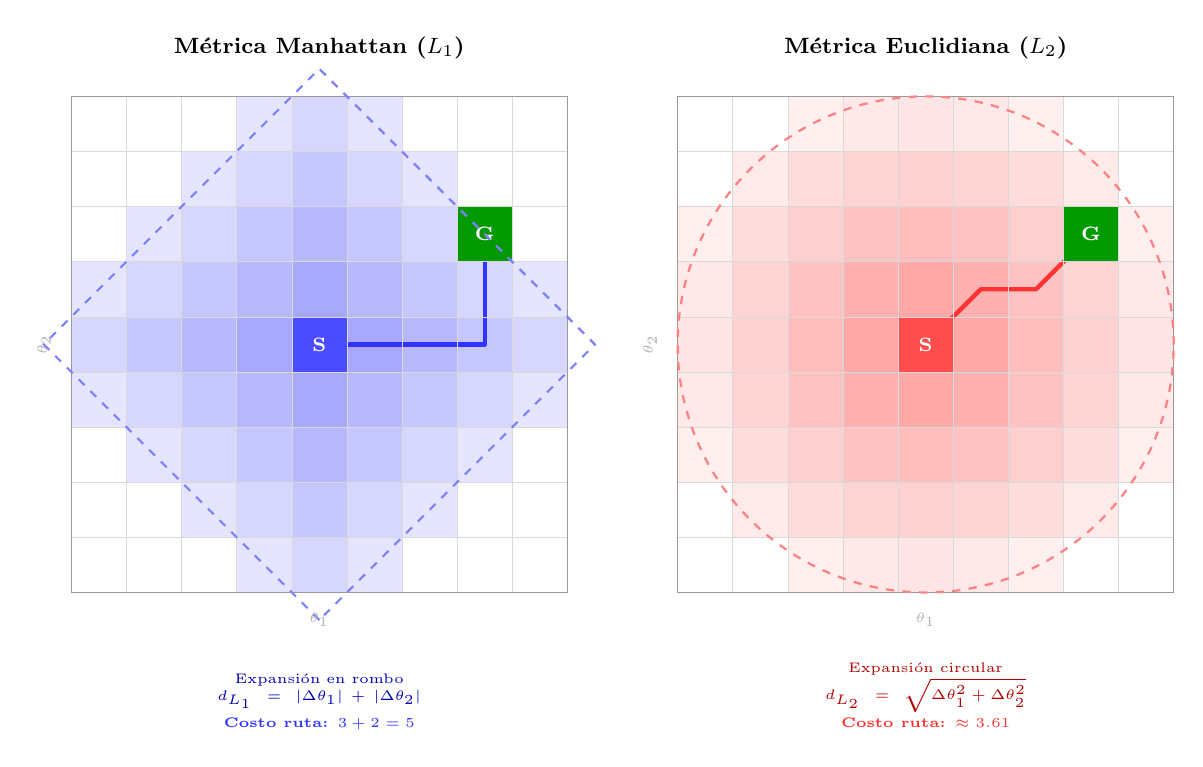
\begin{tikzpicture}[>=stealth, scale=0.7, every node/.style={font=\small}]

% Tamaño de la rejilla
\def\gridsize{9}
% Centro del inicio: celda (4,4), punto medio (4.5,4.5)
% Objetivo: celda (7,6), punto medio (7.5,6.5)

% =============================================
% PANEL IZQUIERDO: Métrica Manhattan (L1)
% =============================================
\begin{scope}[shift={(-6,0)}]
    \node[anchor=south, font=\bfseries\footnotesize] at (4.5, 9.5) {Métrica Manhattan ($L_1$)};
    
    % Rejilla de fondo
    \draw[gray!20, very thin] (0,0) grid (\gridsize,\gridsize);
    
    % Nodos expandidos en forma de rombo (diamante)
    % Centro en celda (4,4). Distancia Manhattan a G(7,6) = |7-4|+|6-4| = 5
    \foreach \x in {0,...,8} {
        \foreach \y in {0,...,8} {
            \pgfmathsetmacro{\mdist}{abs(\x-4) + abs(\y-4)}
            \pgfmathsetmacro{\opac}{max(0, min(35, 40 - 6*\mdist))}
            \ifdim \mdist pt < 5.5pt
                \fill[blue!\opac!white] (\x,\y) rectangle ++(1,1);
            \fi
        }
    }
    
    % Ruta Manhattan: S(4,4) → derecha hasta (7,4) → arriba hasta (7,6) → G
    \draw[blue!80, ultra thick, ->, line cap=round, line join=round] 
        (4.5,4.5) -- (7.5,4.5) -- (7.5,6.5);
    
    % Nodo central (inicio)
    \fill[blue!70] (4,4) rectangle ++(1,1);
    \node[font=\scriptsize\bfseries, white] at (4.5,4.5) {S};
    
    % Nodo objetivo
    \fill[green!60!black] (7,6) rectangle ++(1,1);
    \node[font=\scriptsize\bfseries, white] at (7.5,6.5) {G};
    
    % Redibujar rejilla
    \draw[gray!30, very thin] (0,0) grid (\gridsize,\gridsize);
    \draw[black!40, thin] (0,0) rectangle (\gridsize,\gridsize);
    
    % Contorno del rombo (radio 5, centrado en 4.5,4.5)
    \draw[blue!50, thick, dashed] 
        (4.5,-0.5) -- (-0.5,4.5) -- (4.5,9.5) -- (9.5,4.5) -- cycle;
    
    % Etiquetas de ejes
    \node[font=\tiny, gray!60] at (4.5,-0.5) {$\theta_1$};
    \node[font=\tiny, gray!60, rotate=90] at (-0.5,4.5) {$\theta_2$};
    
    % Anotación
    \node[anchor=north, font=\tiny, text=blue!70!black, text width=4cm, align=center] at (4.5, -1.3) {Expansión en rombo\\$d_{L_1} = |\Delta\theta_1| + |\Delta\theta_2|$};
    
    % Costo de la ruta
    \node[anchor=north, font=\tiny\bfseries, text=blue!80] at (4.5, -2.1) {Costo ruta: $3 + 2 = 5$};
\end{scope}

% =============================================
% PANEL DERECHO: Métrica Euclidiana (L2)
% =============================================
\begin{scope}[shift={(5,0)}]
    \node[anchor=south, font=\bfseries\footnotesize] at (4.5, 9.5) {Métrica Euclidiana ($L_2$)};
    
    % Rejilla de fondo
    \draw[gray!20, very thin] (0,0) grid (\gridsize,\gridsize);
    
    % Nodos expandidos en forma circular
    % Centro en celda (4,4). Distancia Euclidiana a G(7,6) = sqrt(9+4) ≈ 3.61
    \foreach \x in {0,...,8} {
        \foreach \y in {0,...,8} {
            \pgfmathsetmacro{\edist}{sqrt((\x-4)^2 + (\y-4)^2)}
            \pgfmathsetmacro{\opac}{max(0, min(35, 42 - 8*\edist))}
            \ifdim \edist pt < 4.5pt
                \fill[red!\opac!white] (\x,\y) rectangle ++(1,1);
            \fi
        }
    }
    
    % Ruta Euclidiana: más directa (diagonal)
    \draw[red!80, ultra thick, ->, line cap=round, line join=round] 
        (4.5,4.5) -- (5.5,5.5) -- (6.5,5.5) -- (7.5,6.5);
    
    % Nodo central (inicio)
    \fill[red!70] (4,4) rectangle ++(1,1);
    \node[font=\scriptsize\bfseries, white] at (4.5,4.5) {S};
    
    % Nodo objetivo
    \fill[green!60!black] (7,6) rectangle ++(1,1);
    \node[font=\scriptsize\bfseries, white] at (7.5,6.5) {G};
    
    % Redibujar rejilla
    \draw[gray!30, very thin] (0,0) grid (\gridsize,\gridsize);
    \draw[black!40, thin] (0,0) rectangle (\gridsize,\gridsize);
    
    % Contorno del círculo (radio ≈ 4.5, centrado en 4.5,4.5)
    \draw[red!50, thick, dashed] (4.5,4.5) circle (4.5);
    
    % Etiquetas de ejes
    \node[font=\tiny, gray!60] at (4.5,-0.5) {$\theta_1$};
    \node[font=\tiny, gray!60, rotate=90] at (-0.5,4.5) {$\theta_2$};
    
    % Anotación
    \node[anchor=north, font=\tiny, text=red!70!black, text width=4cm, align=center] at (4.5, -1.1) {Expansión circular\\$d_{L_2} = \sqrt{\Delta\theta_1^2 + \Delta\theta_2^2}$};
    
    % Costo de la ruta
    \node[anchor=north, font=\tiny\bfseries, text=red!80] at (4.5, -2.1) {Costo ruta: $\approx 3.61$};
\end{scope}

\end{tikzpicture}


    \caption{Comparativa visual del patrón de expansión de nodos en el algoritmo A* utilizando la métrica de Manhattan ($L_1$) frente a la métrica Euclidiana ($L_2$).}
    \label{fig:comparativa_metricas_Astar}
\end{figure}

Por otro lado, el espacio de configuración para un robot de $n$ articulaciones de revolución libres se 
modela topológicamente como el Toro $T^n$ \parencite{farber2008}. Como se estableció previamente, 
este espacio continuo puede parametrizarse computacionalmente como un hipercubo $I^n$ donde las caras 
opuestas se encuentran matemáticamente identificadas en los límites angulares $[0, 2\pi)$ \parencite{lavalle2006planning}.

Si las métricas $L_1$ o $L_2$ se calculan de forma ingenua como si el 
espacio fuera $\mathbb{R}^n$, la heurística podría violar la condición de admisibilidad al 
sobreestimar el costo cuando la trayectoria más corta realmente atraviesa el borde de 
la parametrización \parencite{lavalle2006planning}. Para respetar la estructura intrínseca de la variedad, 
la heurística debe calcular la distancia integrando el efecto \textit{wrap-around}. 

Para una articulación circular individual ($S^1$), se deben comparar los ángulos evaluando 
el atajo a través de la frontera. Esto exige la inserción de una función de mínimo en el
cálculo para reflejar la identificación de los extremos \parencite{lavalle2006planning}:

$$ \rho(\theta_1, \theta_2) = \min(|\theta_1 - \theta_2|, 2\pi - |\theta_1 - \theta_2|) $$

Al extender esta lógica sobre cada copia de $S^1$ usando las reglas del producto cartesiano 
para construir el Toro $T^n$, las funciones heurísticas se formulan rigurosamente como:

\begin{itemize}
\item \textbf{Heurística $L_1$ en $T^n$:} 
$$\hat{h}(x, y) = \sum_{i=1}^n \min(|x_i - y_i|, 2\pi - |x_i - y_i|)$$
\item \textbf{Heurística $L_2$ en $T^n$:} 
$$\hat{h}(x, y) = \sqrt{\sum_{i=1}^n \min(|x_i - y_i|, 2\pi - |x_i - y_i|)^2}$$
\end{itemize}

La implementación de estas métricas modulares asegura que el algoritmo reconozca 
matemáticamente que el espacio carece de fronteras perimetrales. Así, el planificador 
preserva tanto la admisibilidad de la heurística como la consistencia topológica, lo cual es estrictamente 
necesario para que $A^*$ encuentre la trayectoria óptima que cruza de un lado al otro del espacio 
de estados sin colisiones.


\subsection{Búsqueda estocástica: Algoritmo RRT y completitud probabilística}
% % - Fundamentos matemáticos del muestreo aleatorio en variedades.
% % - Ventajas del RRT para sortear la "maldición de la dimensionalidad" y lidiar con geometrías de colisión complejas donde la retícula determinista de A* resulta ineficiente.

Dado que el espacio de configuraciones continuo $\mathcal{C}$ contiene una infinidad 
no numerable de estados, es imposible que un algoritmo lo evalúe en su totalidad. 
Para que una búsqueda computacional sea representativa, requiere de una secuencia de muestras 
topológicamente densa, lo cual significa que la clausura del conjunto de muestras generadas debe 
ser igual al espacio total. Matemáticamente, una secuencia infinita de puntos elegidos de 
forma independiente y aleatoria sobre un espacio acotado garantiza ser densa con probabilidad uno \parencite{lavalle2006planning}.

Al realizar este muestreo probabilístico sobre una variedad topológica 
(como el Toro $T^n$ o $SO(3)$), es matemáticamente imperativo que la función de densidad 
de probabilidad sea uniforme y respete la \textbf{medida de Haar} del grupo de transformaciones, 
evitando así la introducción de sesgos artificiales. Gracias a las 
propiedades de los productos cartesianos que forman estas variedades, generar una muestra 
aleatoria uniforme en el espacio total $\mathcal{C}$ se logra extrayendo muestras independientes 
en cada uno de sus subespacios proyectados (como en cada circunferencia $S^1$), lo 
que facilita enormemente la implementación algorítmica de la aleatoriedad continua \parencite{lavalle2006planning}.

Para explotar este muestreo, el algoritmo de Árboles Aleatorios de Exploración Rápida 
(RRT, por sus siglas en inglés) construye de manera incremental un grafo topológico (un árbol) 
en $\mathcal{C}_{free}$. En cada iteración, el método genera una configuración aleatoria 
$q_{rand}$ a partir de la distribución uniforme, localiza el vértice del árbol más cercano 
a ella ($q_{near}$) e intenta expandir una nueva arista desde $q_{near}$ en dirección 
a $q_{rand}$. Debido a que la secuencia aleatoria subyacente es densa, el árbol RRT termina 
por cubrir exhaustivamente todo el espacio en el límite \parencite{Choset2005}.

El proceso de expansión estocástica de un árbol RRT se define formalmente mediante el siguiente algoritmo:

\vspace{0.3cm}
\noindent\textbf{Algoritmo: Expansión Estocástica RRT en el Toro $T^n$}
\begin{description}
    \item[\textbf{Entradas:}] Configuración inicial $q_{init} \in \mathcal{C}_{free}$, Módulo de colisiones $\mathcal{C}_{obs}$, Paso máximo de expansión $\Delta q$.
    \item[\textbf{Salida:}] Árbol de exploración $\mathcal{T}$.
    
    \item[\textbf{Paso 1 (Inicialización):}] Se crea el árbol $\mathcal{T}$ asignando $q_{init}$ como su nodo raíz.
    
    \item[\textbf{Paso 2 (Iteración):}] Mientras no se alcance la condición de término (ej. número de iteraciones o hallar el objetivo):
    \begin{enumerate}
        \item \textbf{Muestreo Estocástico:} Se genera una muestra $q_{rand}$ uniformemente bajo la Medida de Haar en $T^n$. Si $q_{rand} \in \mathcal{C}_{obs}$, se descarta y se repite el paso.
        \item \textbf{Localización de Vecindad:} Se identifica el nodo $q_{near} \in \mathcal{T}$ cuya distancia hacia $q_{rand}$ sea la mínima calculada operando con la métrica toroidal ($L_1$ o $L_2$).
        \item \textbf{Extensión Local:} Se genera un nuevo nodo $q_{new}$ avanzando desde $q_{near}$ en dirección a $q_{rand}$, respetando la magnitud de paso $\Delta q$.
        \item \textbf{Validación Segura:} Si el segmento de trayectoria continuo que conecta $q_{near}$ con $q_{new}$ es disjunto de $\mathcal{C}_{obs}$, se añade $q_{new}$ al árbol $\mathcal{T}$ junto con la arista originada en $q_{near}$.
    \end{enumerate}
    
    \item[\textbf{Paso 3 (Retorno):}] Se finaliza el algoritmo y se devuelve la estructura $\mathcal{T}$ consolidada.
\end{description}
\vspace{0.3cm}

Este comportamiento otorga al algoritmo una propiedad matemática fundamental conocida como 
completitud probabilística: si existe una trayectoria solución válida para el problema, 
la probabilidad de que el algoritmo la encuentre converge a uno a medida que la cantidad de 
iteraciones, o el tiempo de ejecución, tiende a infinito \parencite{Choset2005}.

En contraste, los enfoques de búsqueda discreta tradicional, como el algoritmo A* operando 
sobre una retícula ortogonal, sufren severamente por la \enquote{maldición de la dimensionalidad}. En un espacio 
de dimensión $n$, una discretización fina produce un crecimiento exponencial de vértices; por 
ejemplo, una cuadrícula puede generar fácilmente del orden de $100^n$ puntos dentro de una 
región confinada. Si durante la búsqueda el algoritmo determinista se topa con un mínimo local topológico 
(como un obstáculo en forma de \enquote{cuenco} o trampa), desperdiciará una cantidad astronómica de 
recursos evaluando exhaustivamente todos los nodos dentro de esa cavidad antes de poder escapar \parencite{lavalle2006planning}.

Además, en entornos del mundo real, la geometría física del robot y los obstáculos suele estar 
compuesta por miles de primitivas poligonales o mallas no convexas. Calcular 
matemáticamente las fronteras exactas de la región de colisión ($\mathcal{C}_{obs}$) en 
tales geometrías constituye un proceso analítico intratable e ineficiente \parencite{lavalle2006planning}. 

El RRT sortea esta ineficiencia al abandonar la construcción explícita de $\mathcal{C}_{obs}$ 
y tratar la detección de colisiones como una \enquote{caja negra} que solo valida segmentos locales. 
Al generar muestras aleatoriamente y expandir el árbol hacia regiones inexploradas, 
el algoritmo logra evadir de manera natural los mínimos locales de alta dimensionalidad. 
Esta arquitectura, sesgada hacia la exploración del espacio vacío, permite resolver 
problemas de planificación en variedades complejas y escenarios donde los planificadores deterministas 
de retícula resultarían computacionalmente inoperantes \parencite{lavalle2006planning, Choset2005}.

% \subsubsection{Integración y visualización algorítmica en RViz2}
% % - Fundamentos de la comunicación por nodos (middleware) en ROS2 para transmitir las coordenadas calculadas.
% % - Uso de RViz2 como entorno de validación visual puramente matemática, separando la trayectoria teórica de la simulación física.

\subsection{Integración y visualización algorítmica en RViz2}

Para que la trayectoria continua generada en el espacio de configuraciones 
($\mathcal{C}_{free}$) sea útil en la práctica, debe ser transmitida y validada 
computacionalmente antes de su ejecución física. En la arquitectura propuesta, este 
puente entre la abstracción matemática pura y la validación aplicada se logra utilizando 
el ecosistema de ROS2 y su entorno de visualización tridimensional, RViz2.

Desde el punto de vista arquitectónico, ROS2 adopta un enfoque de sistemas distribuidos en el 
que los problemas complejos se dividen en componentes modulares y funcionalmente independientes 
llamados nodos. La comunicación subyacente entre estos nodos está gobernada por un 
\textit{middleware} basado en el estándar industrial DDS (\textit{Data Distribution Service}), el cual 
garantiza una transmisión de datos segura y robusta \parencite{macenski2022robot}.

Para transmitir las coordenadas calculadas por el algoritmo de planificación (la ruta que debe 
seguir el robot), el sistema utiliza un patrón de comunicación asíncrona de 
publicación-suscripción a través de canales conocidos como \textbf{tópicos} (\textit{topics}) \parencite{macenski2022robot}. 
Matemáticamente, la trayectoria discreta extraída del grafo de búsqueda se convierte en 
una secuencia temporal de estados articulares. El nodo planificador (\enquote{custom}) publica estas 
secuencias —usualmente a través del tópico \texttt{joint\_states} y utilizando la estructura 
de transformaciones \texttt{TF} \parencite{chitta2012moveit}— permitiendo que cualquier otro nodo del sistema se suscriba y reciba 
la información topológica actualizada de manera determinista y con muy baja latencia \parencite{macenski2022robot}. 
Esta interconexión de nodos y flujos de datos se describe gráficamente en la Figura \ref{fig:arquitectura_ros2}.

\begin{figure}[htbp]
    \centering
    % !TeX root = ../main.tex
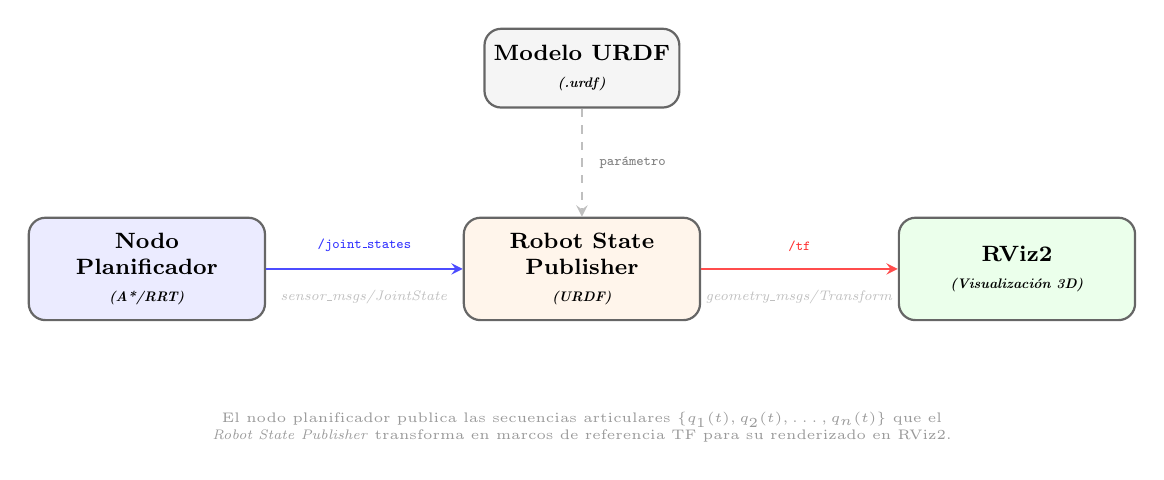
\begin{tikzpicture}[>=stealth, scale=0.85, every node/.style={font=\small},
    % Estilos de nodos
    rosnode/.style={
        draw=black!60, thick, rounded corners=6pt,
        fill=white, minimum width=3.0cm, minimum height=1.3cm,
        font=\footnotesize\bfseries, align=center
    },
    rostopic/.style={
        font=\tiny\ttfamily, fill=white, inner sep=2pt
    }
]

% =============================================
% NODOS ROS2
% =============================================

% Nodo Planificador (izquierda)
\node[rosnode, fill=blue!8] (planner) at (-6.5, 0) 
    {Nodo\\Planificador\\{\tiny\textit{(A*/RRT)}}};

% Robot State Publisher (centro)
\node[rosnode, fill=orange!8] (rsp) at (0, 0) 
    {Robot State\\Publisher\\{\tiny\textit{(URDF)}}};

% RViz2 (derecha)
\node[rosnode, fill=green!8] (rviz) at (6.5, 0) 
    {RViz2\\{\tiny\textit{(Visualización 3D)}}};

% Nodo URDF/modelo (arriba del RSP)
\node[rosnode, fill=gray!8, minimum width=2.4cm, minimum height=1cm] (urdf) at (0, 3) 
    {Modelo URDF\\{\tiny\textit{(.urdf)}}};

% =============================================
% CONEXIONES (Tópicos)
% =============================================

% Planificador → RSP via /joint_states
\draw[->, thick, blue!70] (planner.east) -- (rsp.west)
    node[rostopic, midway, above=4pt, text=blue!80] {/joint\_states}
    node[midway, below=4pt, font=\tiny, gray!50] {\textit{sensor\_msgs/JointState}};

% RSP → RViz2 via /tf
\draw[->, thick, red!70] (rsp.east) -- (rviz.west)
    node[rostopic, midway, above=4pt, text=red!80] {/tf}
    node[midway, below=4pt, font=\tiny, gray!50] {\textit{geometry\_msgs/Transform}};

% URDF → RSP (parámetro)
\draw[->, thick, gray!50, dashed] (urdf.south) -- (rsp.north)
    node[rostopic, midway, right=4pt, text=black!50] {parámetro};

% =============================================
% NOTA DESCRIPTIVA
% =============================================
\node[anchor=north, font=\tiny, text=black!40, text width=12cm, align=center] at (0, -2.0) 
    {El nodo planificador publica las secuencias articulares $\{q_1(t), q_2(t), \dots, q_n(t)\}$ que el \textit{Robot State Publisher} transforma en marcos de referencia TF para su renderizado en RViz2.};

\end{tikzpicture}


    \caption{Arquitectura de comunicación en ROS2 para la traducción y visualización geométrica de las trayectorias.}
    \label{fig:arquitectura_ros2}
\end{figure}

Antes de introducir variables dinámicas complejas (como masa, inercia, gravedad o fricción) 
en un simulador físico completo (como Gazebo \parencite{macenski2022robot}), es una práctica imperativa validar 
la consistencia estrictamente geométrica de la trayectoria. 

Es aquí donde entra en juego RViz2. A diferencia de un motor de física de caja rígida, 
RViz2 actúa como un \textbf{renderizador tridimensional interactivo} y una herramienta de 
introspección de datos. RViz2 proporciona un entorno de validación visual puramente 
matemático: se suscribe directamente a los tópicos de estados articulares publicados 
por el planificador y aplica el mapeo cinemático directo para proyectar la curva abstracta 
de $\mathcal{C}_{free}$ en el espacio de trabajo euclidiano real ($\mathbb{R}^3$) \parencite{chitta2012moveit}.

Para materializar este mapeo cinemático de forma automatizada, el sistema depende de un 
componente estructural indispensable: el formato estandarizado URDF (\textit{Unified Robot 
Description Format}). Este archivo actúa como el nexo definitivo entre la abstracción topológica 
y la ingeniería física, ya que codifica explícitamente la descripción geométrica, la 
jerarquía de eslabones y los ejes de revolución del manipulador. Es a partir de esta parametrización 
que el \textit{middleware} de ROS2 es capaz de instanciar y resolver el árbol de 
transformaciones espaciales (\texttt{TF}), permitiendo que el vector de estado puramente 
matemático publicado por el algoritmo adquiera volumen y sentido espacial dentro del entorno visual.

Esta separación metodológica entre la trayectoria teórica y la simulación física es crucial 
por varias razones:
\begin{itemize}
\item \textbf{Aislamiento de errores:} Al aislar la cinemática de la dinámica, el diseñador puede 
observar gráficamente si el algoritmo de planificación funciona. Si el brazo robótico 
atraviesa un obstáculo en RViz2, el error radica inequívocamente en la definición matemática 
de la región de colisión ($\mathcal{C}_{obs}$) o en la heurística del algoritmo de búsqueda 
discreto.
\item \textbf{Identificación de inestabilidades topológicas:} Permite verificar de forma visual si 
la trayectoria sufre de \enquote{saltos} articulares (discontinuidades debidas a la topología no 
contráctil del Toro $T^n$) antes de que dichos comportamientos se envíen a un simulador físico o a 
un controlador real, lo cual podría causar un comportamiento caótico.
\end{itemize}

En definitiva, la integración con los nodos de ROS2 y la visualización en RViz2 
proporcionan una prueba fundamental de que el problema de búsqueda abstracta sobre 
la variedad topológica se ha resuelto de manera consistente y segura, todo ello antes de 
comprometer hardware real o simulaciones de alta fidelidad física.

\section{Análisis diferencial y seguridad cinemática}
% % NOTA DE ESTRATEGIA: El cierre maestro. Conectas la topología con la cinemática de los ingenieros, 
% % validando que tu modelo matemático asegura que el robot físico no "colapse" o se vuelva inestable.

Una vez que los algoritmos de planificación han trazado una ruta topológicamente viable en el 
espacio de configuraciones, es imperativo garantizar que su ejecución física sea mecánicamente segura 
y estable. Esta sección establece el puente analítico definitivo entre la abstracción matemática y el 
control del manipulador. Para lograrlo, se aborda el estudio del mapa cinemático desde la perspectiva 
de la geometría diferencial, formalizando la relación continua entre el movimiento articular y el 
espacio de trabajo euclidiano. A partir de esta base, se explora el papel de la matriz Jacobiana y 
el Teorema de la Función Inversa en la propagación de velocidades. Finalmente, se analizan las 
singularidades cinemáticas no solo como pérdidas de grados de libertad mecánicos, sino como 
inestabilidades topológicas inherentes a la variedad, demostrando que el análisis diferencial riguroso 
es clave para prevenir comportamientos caóticos durante el movimiento del robot.


\subsection{El mapa cinemático como aplicación diferencial}
% % - Formalización de la cinemática directa e inversa como funciones continuas entre la variedad de configuración 
% % (T^n) y el espacio de trabajo euclidiano (\mathbb{R}^3).

Para poder operar en el mundo físico, es matemáticamente necesario traducir el estado interno 
de las articulaciones del robot a las coordenadas espaciales de su herramienta. El problema 
de la cinemática directa consiste, precisamente, en calcular la posición del efector final en 
función de estas configuraciones articulares \parencite{grant2015topology}. 

Si modelamos el espacio de configuraciones del robot como la variedad 
topológica $\mathcal{C}$ (que para un brazo articulado de $n$ grados de revolución sin 
restricciones de límites corresponde al Toro $T^n$) y denotamos como $\mathcal{W}$ al 
espacio de trabajo euclidiano (típicamente un subespacio de $\mathbb{R}^3$), la posición del 
efector final depende de las configuraciones de manera continua. Por consiguiente, 
la cinemática directa se formaliza rigurosamente como una función continua 
$F: \mathcal{C} \to \mathcal{W}$ (a menudo denotada también como $\phi: Q \to M$ en geometría 
diferencial), a la cual se le conoce como el mapa del efector final o mapa cinemático \parencite{grant2015topology}.

Bajo el enfoque de la geometría diferencial, al tratarse de variedades suaves, el movimiento del 
sistema nos permite relacionar las velocidades en ambos espacios tomando derivadas respecto 
al tiempo. La velocidad euclidiana del efector, $\dot{x}$, se relaciona con las velocidades 
articulares, $\dot{q}$, mediante la ecuación diferencial $\dot{x} = J(q)\dot{q}$, en donde $J(q)$ 
representa la matriz Jacobiana de la función $\phi$, identificada formalmente como el 
diferencial de la aplicación, $D\phi$ \parencite{choset2005principles}.

Por el contrario, el problema de la cinemática inversa radica en encontrar todas las 
configuraciones articulares en $\mathcal{C}$ que permiten lograr una posición y 
orientación específica del efector final en $\mathcal{W}$. Teóricamente, esto requiere 
construir una función de mapa inverso $I: \mathcal{W} \to \mathcal{C}$ que satisfaga 
la identidad $F(I(w)) = w$ para todo punto $w \in \mathcal{W}$ \parencite{grant2015topology}.

Aquí es donde la topología impone una limitación fundamental. A menudo ocurre que la variedad 
de configuración $\mathcal{C}$ (como el Toro $T^n$) y la variedad del espacio de 
trabajo $\mathcal{W}$ (incrustado en $\mathbb{R}^3$) tienen dimensiones o estructuras 
intrínsecas diferentes, por lo que \textbf{no son homeomorfos}. Esta falta de equivalencia topológica 
hace que las aplicaciones cinemáticas inversas, $\phi^{-1}$, raramente sean homeomorfismos, 
incluso si los espacios coinciden en sus dimensiones \parencite{choset2005principles}. 

Físicamente, esto se manifiesta de dos maneras:
\begin{itemize}
\item \textbf{Pérdida de inyectividad:} La aplicación inversa suele ser una función \enquote{uno a varios}. 
Para una misma coordenada euclidiana en el espacio de trabajo, a menudo existen múltiples 
soluciones en la variedad de configuración, lo que permite al sistema adoptar posturas 
físicamente distintas (como las configuraciones conocidas como \enquote{codo-arriba} o \enquote{codo-abajo}, ilustradas en la Figura \ref{fig:codo_arriba_abajo}) 
para el mismo punto final \parencite{choset2005principles}.
\item \textbf{Inexistencia de funciones continuas globales:} En ciertos mecanismos, como juntas universales 
donde el espacio de trabajo es una esfera ($S^2$) y el de configuraciones un Toro ($T^2$), 
la topología algebraica demuestra que \textbf{una aplicación cinemática inversa global y continua 
matemáticamente no puede existir}. Cualquier intento de forzar una función inversa continua 
generaría contradicciones en la transformación de los grupos de homotopía entre ambos espacios \parencite{grant2015topology}.
\end{itemize}

\begin{figure}[htbp]
    \centering
    % !TeX root = ../main.tex
\usetikzlibrary{intersections, calc}

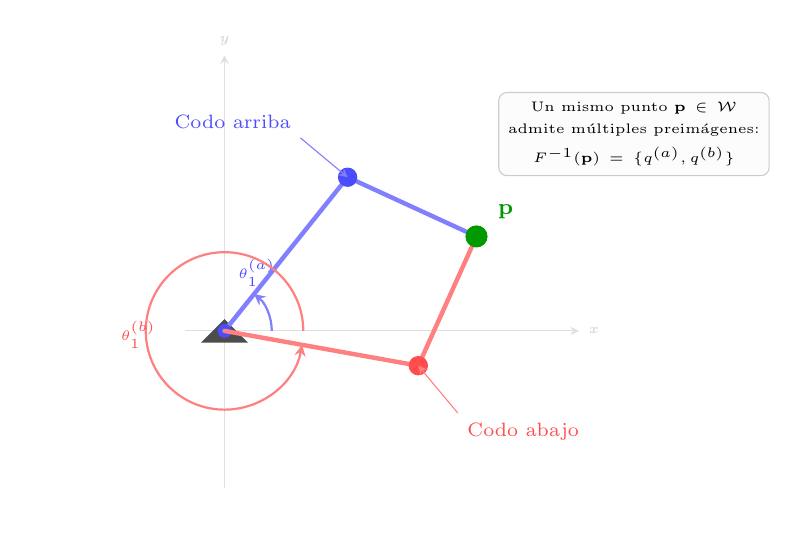
\begin{tikzpicture}[>=stealth, scale=1.0, every node/.style={font=\small}]

% 1. DEFINICIÓN DE PARÁMETROS
\coordinate (J0) at (0,0);           % Base
\coordinate (target) at (3.2, 1.2);  % Punto P objetivo
\def\lone{2.5}                       % Longitud eslabón 1
\def\ltwo{1.8}                       % Longitud eslabón 2

% 2. CÁLCULO AUTOMÁTICO DE LOS CODOS (Intersección de dos círculos)
\path[name path=c1] (J0) circle (\lone);
\path[name path=c2] (target) circle (\ltwo);
\path[name intersections={of=c1 and c2, by={J1up, J1down}}];

% --- Ejes y Base ---
\draw[->, gray!25] (-0.5,0) -- (4.5,0) node[right, font=\tiny, gray!40] {$x$};
\draw[->, gray!25] (0,-2) -- (0,3.5) node[above, font=\tiny, gray!40] {$y$};
\fill[black!70] (-0.3,-0.15) -- (0.3,-0.15) -- (0,0.15) -- cycle;

% =============================================
% CONFIGURACIÓN AZUL (Codo Arriba)
% =============================================
\draw[ultra thick, blue!50, line cap=round] (J0) -- (J1up) -- (target);
\fill[blue!70] (J0) circle (2.5pt);
\fill[blue!70] (J1up) circle (3.5pt);

% Etiqueta Codo Arriba (flecha TikZ nativa, sin triángulos manuales)
\draw[<-, blue!50, thin] (J1up) -- ++(-0.6, 0.5);
\node[blue!70, font=\scriptsize, anchor=south east] at ($(J1up)+(-0.6, 0.5)$) {Codo arriba};

% Arco θ₁(a) — radio pequeño, desde el eje x hasta el eslabón 1
% Ángulo calculado: atan2(y,x) de J1up relativo a J0
\pgfmathanglebetweenpoints{\pgfpointanchor{J0}{center}}{\pgfpointanchor{J1up}{center}}
\edef\angleUp{\pgfmathresult}
\draw[->, blue!50, thick] (0.6,0) arc (0:\angleUp:0.6);
\node[blue!70, font=\tiny, anchor=south] at ({0.5*cos(35)},{0.5*sin(35)+0.15}) {$\theta_1^{(a)}$};

% =============================================
% CONFIGURACIÓN ROJA (Codo Abajo)
% =============================================
\draw[ultra thick, red!50, line cap=round] (J0) -- (J1down) -- (target);
\fill[red!70] (J1down) circle (3.5pt);

% Etiqueta Codo Abajo (flecha TikZ nativa)
\draw[<-, red!50, thin] (J1down) -- ++(0.5, -0.6);
\node[red!70, font=\scriptsize, anchor=north west] at ($(J1down)+(0.5, -0.6)$) {Codo abajo};

% Arco θ₁(b) — radio más grande para no solapar con el azul
\pgfmathanglebetweenpoints{\pgfpointanchor{J0}{center}}{\pgfpointanchor{J1down}{center}}
\edef\angleDown{\pgfmathresult}
% Si el ángulo es negativo (codo abajo del eje x), dibujar hacia abajo
\draw[->, red!50, thick] (1.0,0) arc (0:\angleDown:1.0);
\node[red!70, font=\tiny] at ({1.1*cos(\angleDown/2)},{1.1*sin(\angleDown/2)-0.15}) {$\theta_1^{(b)}$};

% =============================================
% PUNTO P (Objetivo)
% =============================================
\fill[green!60!black] (target) circle (4pt);
\node[green!60!black, font=\footnotesize\bfseries, anchor=south west] at ($(target)+(0.15, 0.1)$) {$\mathbf{p}$};

% =============================================
% ANOTACIÓN LATERAL
% =============================================
\node[draw=black!20, rounded corners=3pt, fill=gray!2, 
      font=\tiny, text width=3.2cm, align=center] at (5.2, 2.5) {
    Un mismo punto $\mathbf{p} \in \mathcal{W}$\\[2pt]
    admite múltiples preimágenes:\\[3pt]
    $F^{-1}(\mathbf{p}) = \{q^{(a)}, q^{(b)}\}$
};

\end{tikzpicture}

    \caption{Pérdida de inyectividad en el mapa cinemático inverso: múltiples configuraciones articulares (\enquote{codo-arriba} y \enquote{codo-abajo}) correspondientes a una misma coordenada en el espacio de trabajo.}
    \label{fig:codo_arriba_abajo}
\end{figure}

Debido a estas propiedades, mientras que el mapa cinemático directo $F$ es una función continua 
bien comportada y determinista que mapea del Toro a $\mathbb{R}^3$, la cinemática inversa sufre 
inestabilidades topológicas que fuerzan a los algoritmos computacionales a operar únicamente 
sobre vecindades locales o mediante técnicas de Jacobiano inverso.

\subsection{Singularidades y el teorema de la función inversa}
% % - Definición del Jacobiano como la derivada del mapa cinemático.
% % - Uso del Teorema de la Función Inversa para explicar analíticamente la pérdida de rango (singularidades cinemáticas).
% % - Propósito final: Vincular esta falla matemática con las inestabilidades topológicas mencionadas en 2.2.3 (ej. Gimbal-lock).

Como se estableció anteriormente, el mapa cinemático (o cinemática directa) 
$\phi: Q \to M$ relaciona el espacio de configuraciones con el espacio de trabajo. 
Para comprender cómo se transfiere el movimiento entre ambos espacios, es necesario 
relacionar sus velocidades. Al derivar esta función respecto al tiempo, se obtiene la 
relación entre el vector de velocidades articulares $\dot{q}$ y el vector de velocidades 
del efector final $\dot{x}$, expresada mediante la ecuación $\dot{x} = J(q)\dot{q}$. 
La matriz $J(q) = \frac{\partial \phi}{\partial q}$ representa el diferencial de esta aplicación 
y es fundamental en la cinemática diferencial, conociéndose comúnmente en la robótica como la 
\textbf{matriz Jacobiana} \parencite{choset2005principles}. 

Para que un robot pueda moverse y rotar libremente en todas las direcciones posibles de su 
espacio de trabajo, la matriz Jacobiana debe tener rango máximo \parencite{lynch2017modern}. Desde el análisis matemático, 
el \textit{Teorema de la Función Inversa} establece que una función diferenciable posee una inversa 
local continua si y solo si su matriz Jacobiana es invertible (es decir, posee rango completo). 

Sin embargo, existen configuraciones específicas del robot en las que la matriz Jacobiana 
falla en mantener este rango máximo \parencite{lynch2017modern}. A estas posturas se les denomina \textbf{singularidades 
cinemáticas}. Cuando el Jacobiano pierde rango, el Teorema de la Función Inversa deja de 
ser aplicable y el mapeo inverso colapsa analíticamente. Físicamente, esto significa que el 
conjunto multidimensional de velocidades articulares $\dot{q}$ se mapea a un conjunto de menor 
dimensión en el espacio de velocidades del efector final $\dot{x}$. Como resultado, el efector 
final pierde la capacidad de moverse o rotar en una o más direcciones, volviendo físicamente imposible el 
movimiento instantáneo sobre esos ejes \parencite{choset2005principles, lynch2017modern}.

Esta falla matemática y analítica local está profundamente vinculada con las inestabilidades 
topológicas globales mencionadas en secciones anteriores. Un ejemplo clásico e histórico de 
esta pérdida de rango es el \textit{gimbal-lock} (bloqueo del cardán), un fenómeno que afectó 
incluso a las misiones espaciales Apollo. El \textit{gimbal-lock} se define como la pérdida de un 
grado de libertad de movimiento que ocurre cuando, tras una sucesión de rotaciones, dos 
ejes de un mecanismo se alinean en el mismo plano \parencite{Mosquera2017}. 

Topológicamente, el \textit{gimbal-lock} no es un mero defecto de diseño mecánico, sino una consecuencia 
inevitable de la geometría del espacio: se produce porque \textbf{no existe un algoritmo de 
planificación de movimientos estable y global} sobre la variedad de rotaciones tridimensionales 
$SO(3)$ \parencite{Mosquera2017}. Cuando un robot se acerca a una singularidad cinemática, la pérdida de rango en el 
Jacobiano impide calcular la cinemática inversa de manera estable y continua. Si el algoritmo 
de control intenta forzar el movimiento a través de esta singularidad, la imposibilidad 
matemática de invertir la matriz desencadena exactamente las discontinuidades topológicas 
predichas por el Teorema de Farber, provocando que el mecanismo sufra \enquote{saltos} articulares 
impredecibles y un comportamiento inestable \parencite{lynch2017modern}.

\begin{figure}[htbp]
    \centering
    % !TeX root = ../main.tex
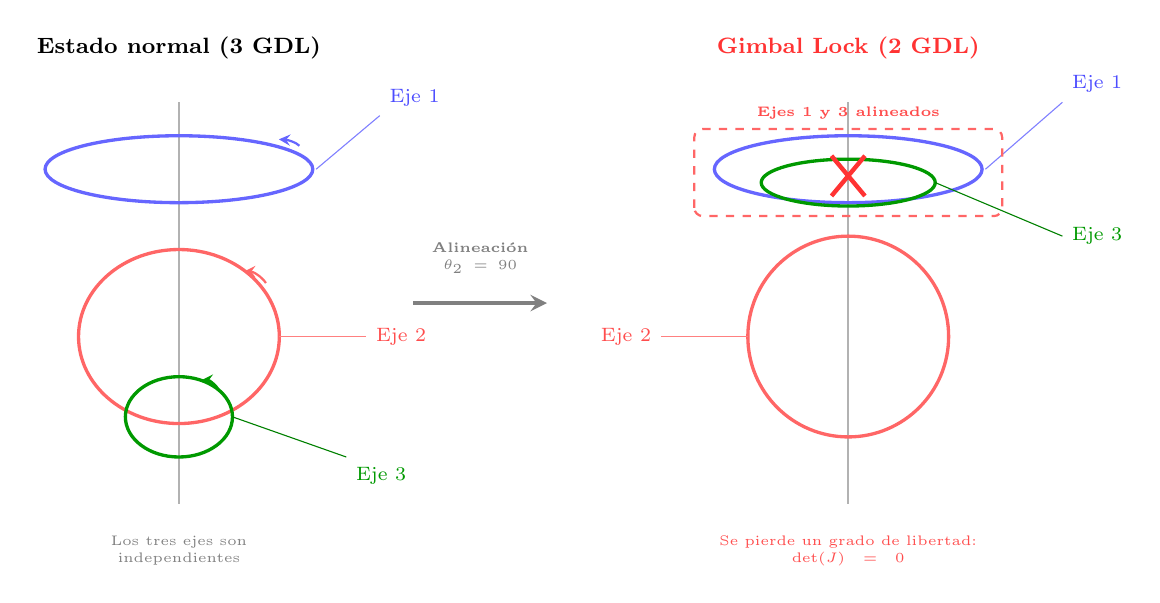
\begin{tikzpicture}[>=stealth, scale=0.85, every node/.style={font=\small}]

% =============================================
% PANEL IZQUIERDO: Estado Normal (3 GDL)
% =============================================
\begin{scope}[shift={(-5,0)}]
    \node[anchor=south, font=\bfseries\footnotesize] at (0, 4.0) {Estado normal (3 GDL)};
    
    % Eje vertical principal
    \draw[black!30, thick] (0,-2.5) -- (0,3.5);
    
    % Anillo exterior (Yaw) - arriba
    \draw[blue!60, very thick] (0,2.5) ellipse (2 and 0.5);
    \draw[->, blue!60, thick] (1.8,2.85) arc[start angle=20, end angle=80, x radius=0.4, y radius=0.15];
    % Etiqueta con línea guía hacia arriba
    \draw[blue!50, thin] (2.05,2.5) -- (3.0,3.3);
    \node[font=\scriptsize, blue!70, anchor=south west] at (3.0,3.3) {Eje 1};
    
    % Anillo medio (Pitch) - centro
    \draw[red!60, very thick] (0,0) ellipse (1.5 and 1.3);
    \draw[->, red!60, thick] (1.3,0.8) arc[start angle=35, end angle=90, radius=0.4];
    % Etiqueta con línea guía a la derecha
    \draw[red!50, thin] (1.5,0) -- (2.8,0);
    \node[font=\scriptsize, red!70, anchor=west] at (2.8,0) {Eje 2};
    
    % Anillo interior (Roll) - abajo
    \draw[green!60!black, very thick] (0,-1.2) ellipse (0.8 and 0.6);
    \draw[->, green!60!black, thick] (0.6,-0.8) arc[start angle=30, end angle=90, radius=0.3];
    % Etiqueta con línea guía abajo
    \draw[green!50!black, thin] (0.8,-1.2) -- (2.5,-1.8);
    \node[font=\scriptsize, green!60!black, anchor=north west] at (2.5,-1.8) {Eje 3};
    
    % Nota
    \node[font=\tiny, black!50, text width=3cm, align=center] at (0,-3.2) {Los tres ejes son\\independientes};
\end{scope}

% =============================================
% FLECHA CENTRAL
% =============================================
\draw[->, ultra thick, black!50] (-1.5,0.5) -- (0.5,0.5);
\node[anchor=south, font=\tiny\bfseries, black!50, text width=1.8cm, align=center] at (-0.5,0.8) {Alineación\\$\theta_2 = 90°$};

% =============================================
% PANEL DERECHO: Gimbal Lock (2 GDL)
% =============================================
\begin{scope}[shift={(5,0)}]
    \node[anchor=south, font=\bfseries\footnotesize, red!80] at (0, 4.0) {Gimbal Lock (2 GDL)};
    
    % Eje vertical principal
    \draw[black!30, thick] (0,-2.5) -- (0,3.5);
    
    % Anillo exterior (Yaw) — arriba
    \draw[blue!60, very thick] (0,2.5) ellipse (2 and 0.5);
    % Etiqueta Eje 1 — arriba a la derecha, bien separada
    \draw[blue!50, thin] (2.05,2.5) -- (3.2,3.5);
    \node[font=\scriptsize, blue!70, anchor=south west] at (3.2,3.5) {Eje 1};
    
    % Anillo interior ALINEADO con el exterior (¡el problema!)
    \draw[green!60!black, very thick] (0,2.3) ellipse (1.3 and 0.35);
    % Etiqueta Eje 3 — abajo a la derecha, separada del Eje 1
    \draw[green!50!black, thin] (1.3,2.3) -- (3.2,1.5);
    \node[font=\scriptsize, green!60!black, anchor=west] at (3.2,1.5) {Eje 3};
    
    % Anillo medio (Pitch) - girado 90° (ahora es un círculo grande)
    \draw[red!60, very thick] (0,0) ellipse (1.5 and 1.5);
    % Etiqueta Eje 2 — a la izquierda
    \draw[red!50, thin] (-1.5,0) -- (-2.8,0);
    \node[font=\scriptsize, red!70, anchor=east] at (-2.8,0) {Eje 2};
    
    % Cruz indicando GDL perdido (sobre la zona alineada)
    \draw[red!80, ultra thick] (-0.25,2.7) -- (0.25,2.1);
    \draw[red!80, ultra thick] (-0.25,2.1) -- (0.25,2.7);
    
    % Recuadro de alerta (solo alrededor de los ejes alineados)
    \draw[red!60, thick, dashed, rounded corners=3pt] (-2.3,1.8) rectangle (2.3,3.1);
    \node[font=\tiny\bfseries, red!70, anchor=south] at (0,3.1) {Ejes 1 y 3 alineados};
    
    % Nota
    \node[font=\tiny, red!70, text width=3.5cm, align=center] at (0,-3.2) {Se pierde un grado de libertad:\\$\det(J) = 0$};
\end{scope}

\end{tikzpicture}


    \caption{Representación del fenómeno de \textit{gimbal-lock}: la alineación de dos ejes cardánicos provoca la pérdida de un grado de libertad, donde $\det(J) = 0$.}
    \label{fig:gimbal_lock}
\end{figure}